\documentclass[12pt]{report}
\usepackage[utf8]{inputenc} 
\usepackage[T1]{fontenc} 

\usepackage{graphicx}
\usepackage{abstract}
\usepackage{mathpazo} 
\usepackage{float}
\usepackage[hyphens]{url}
\usepackage[breaklinks]{hyperref}
\usepackage{amsmath}
\usepackage[normalem]{ulem}
\usepackage{amsfonts}
\useunder{\uline}{\ul}{}
\usepackage{longtable}
\usepackage{verbatim}
\usepackage{adjustbox}
\usepackage{setspace}
\usepackage{indentfirst}
\usepackage{amssymb}
\usepackage{mathtools}
\usepackage{url}
\usepackage{graphicx}
\usepackage{subfig}
\usepackage[nottoc,numbib]{tocbibind}
\usepackage{listings}

\begin{document}

\newtheorem{thm}{Theorem}[section] 
\newtheorem{defn}[thm]{Definition} 
\newtheorem{ex}[thm]{Example}
\newtheorem{pro}[thm] {Proof}
\newtheorem{cor}[thm] {Corollary}
\newtheorem{lem}[thm] {Lemma}
\newtheorem{rmk}[thm] {Remark} 
\newtheorem{prop} [thm] {Proposition}

\newtheorem{theorem}{Theorem}
\newtheorem{acknowledgement}[theorem]{Acknowledgement}
\newtheorem{algorithm}[theorem]{Algorithm}
\newtheorem{axiom}[theorem]{Axiom}
\newtheorem{case}[theorem]{Case}
\newtheorem{claim}[theorem]{Claim}
\newtheorem{conclusion}[theorem]{Conclusion}
\newtheorem{condition}[theorem]{Condition}
\newtheorem{conjecture}[theorem]{Conjecture}
\newtheorem{corollary}[theorem]{Corollary}
\newtheorem{criterion}[theorem]{Criterion}
\newtheorem{definition}[theorem]{Definition}
\newtheorem{example}[theorem]{Example}
\newtheorem{exercise}[theorem]{Exercise}
\newtheorem{lemma}[theorem]{Lemma}
\newtheorem{notation}[theorem]{Notation}
\newtheorem{problem}[theorem]{Problem}
\newtheorem{proposition}[theorem]{Proposition}
\newtheorem{remark}[theorem]{Remark}
\newtheorem{solution}[theorem]{Solution}
\newtheorem{summary}[theorem]{Summary}
\newenvironment{proof}[1][Proof]{\noindent\textbf{#1.} }{\ \rule{0.5em}{0.5em}}

\doublespacing


% Title Page ------------------------------------------
\begin{titlepage} 
	\newcommand{\HRule}{\rule{\linewidth}{0.5mm}} 
	\center 
	
	\textsc{\LARGE Wilfrid Laurier University}\\[1.5cm] % School name
	
	\textsc{\Large MA 680 - Seminar in Mathematical Modelling}\\[0.5cm] % Course name
	
	\textsc{\large Department of Mathematics}\\[0.5cm] % Department name
	
	\HRule\\[0.4cm]
	{\huge\bfseries Dynamic Mode Decomposition}\\[0.4cm] % Document name
	
	\HRule\\[1.5cm]
	\begin{minipage}{0.4\textwidth}
		\begin{flushleft}
			\large
			\textit{Authors}\\
			Austin Sammon \\Timothy Ponepal \\Wayne Shen % Your name
		\end{flushleft}
	\end{minipage}
	~
	\begin{minipage}{0.4\textwidth}
		\begin{flushright}
			\large
			\textit{Instructor}\\
			Dr. Cristina Stoica % Instructor
		\end{flushright}
	\end{minipage}
	\vfill\vfill\vfill
	
	{\large Tuesday December 20, 2022} % Date
	
	\vfill\vfill\vfill
	
\includegraphics[width=0.2\textwidth]{Wlu_colour_logo.jpg}\\[0.1cm] 
	
	\vfill
	
\end{titlepage}

% End of Title Page ------------------------------------

\renewcommand{\abstractname}{Abstract}
\renewcommand{\abstractnamefont}{\normalfont\Huge\bfseries}
\begin{abstract}
Data-driven modelling and control of complex systems represent a quickly advancing field with significant potential that can be applied to a wide array of industrial and academic areas. Dynamic mode decomposition (DMD) is an equation-free and data-driven technique that takes advantage of dimensional reduction and provides a spatiotemporal decomposition of data into a set of dynamic modes. This paper provides a discussion of the theoretical foundation behind DMD including singular value decomposition as well as its connection to the Koopman operator. Additionally, examples of dynamic mode decomposition's application to epidemiology, trading markets, and weather systems are provided, accompanied by an examination of the useful information that can be derived from the output. 

\end{abstract}

\tableofcontents

\makeatletter
\def\@makechapterhead#1{%
  \vspace*{50\p@}% <----------------- Space from top of page to Chapter #
  {\parindent \z@ \raggedright \normalfont
    \ifnum \c@secnumdepth >\m@ne
        \huge\bfseries \thechapter.\ % <-- Chapter # (without "Chapter")
    \fi
    \interlinepenalty\@M
    #1\par\nobreak% <------------------ Chapter title
    \vskip 40\p@% <------------------ Space between the chapter title and first paragraph
  }}
\makeatother

\chapter{Introduction}
In modern society, data can be collected from anywhere at any time. Scientists and mathematicians have been finding ways to analyze and discover a connecting model between each data point. However, with the limitation of computational machines increasing gradually as time proceeded, we are able to take advantage of their computational ability to calculate high-dimensional datasets at different time intervals. Dynamic mode decomposition is an equation-free and complete data-driven mechanism that utilizes the essence of dimensional reduction from a high dimensional measurement into the size of the number of measurements taken. 

\section{Background}
The idea of dynamic mode decomposition was initially introduced by Peter J. Schmid, professor of mechanical engineering at King Abdullah University of Science and Technology, in 2008 in the fluid dynamics society to monitor and extract dynamic features in fluid data.
\begin{figure}
    \centering
    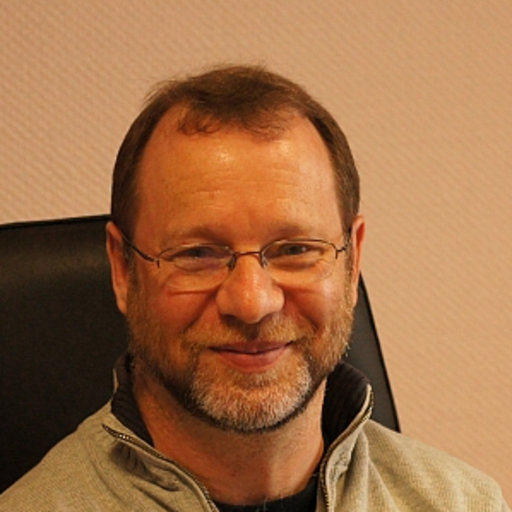
\includegraphics[width=0.5\textwidth]{Peter-Schmid-5.jpg}
    \caption{Peter J. Schmid}
\end{figure}
Clarence W. Rowley later connected dynamic mode decomposition to the non-linear dynamical system, known as Koopman's Theory, in 2009, and DMD has been modified into analyzing non-linear systems.

Due to its simplicity in application, dynamic mode decomposition has been applied to a wide range of categories apart from fluid dynamics, such as disease modelling, plasma, neuroscience, financial trading, etc. In short, DMD can be applied and analyze the system when there exists a collection of data, and predict the future time frame interval.
\newcommand*{\vertbar}{\rule[-1ex]{0.5pt}{2.5ex}}
\[
X = 
\left[
  \begin{array}{cccc}
    \vertbar & \vertbar &        & \vertbar \\
    x_{0}    & x_{1}    & \ldots & x_{m-1}    \\
    \vertbar & \vertbar &        & \vertbar 
  \end{array}
\right]
\]
\[
X' = 
\left[
  \begin{array}{cccc}
    \vertbar & \vertbar &        & \vertbar \\
    x_{1}    & x_{2}    & \ldots & x_{m}    \\
    \vertbar & \vertbar &        & \vertbar 
  \end{array}
\right]
\]

\section{Compact Singular Value Decomposition}
Dynamic mode decomposition is based on singular value decomposition. Singular value decomposition (SVD) is one of the most important decomposition techniques that splits a system into a set of linearly independent components. This is essential for the computation of dimensional reduction that can be utilized in the data-driven mechanism of DMD. In the view of linear algebra, SVD can separate any matrices into a set of low-ranked linearly independent sub-matrices. That is, for $r$ = min($m,n$), any $X_{n\times m}$ matrices can be separated into
\begin{equation}
    X_{n\times m} = U_{n\times r}\Sigma_{r\times r}V^T_{r\times m}
    \label{SVD_Base}
\end{equation}
Where 
\begin{itemize}
    \item $\Sigma_{r\times r}$ is the matrix of the eigenvalues of 
    $\begin{cases}
                X^TX & $if $ n\le m\\
                XX^T & $if $ m\le n
    \end{cases}$
    \item $V_{m\times r}$ is the normalized eigenvectors of 
    $\begin{cases}
                X^TX & $if $ n\le m\\
                XX^T & $if $ m\le n
    \end{cases}$
    \item $U_{n\times r}$ is the multiplication of the inverse of eigenvectors, $X$, and the normalized eigenvectors
\end{itemize}
Example:
\begin{eqnarray*}
X &=&%
\begin{bmatrix}
1 & 0 \\ 
0 & 1 \\
1 & 1
\end{bmatrix}
\end{eqnarray*}
Let $Y = X^TX$,
\begin{eqnarray*}
Y &=&%
\begin{bmatrix}
1 & 0 & 1 \\ 
0 & 1 & 1
\end{bmatrix}%
\begin{bmatrix}
1 & 0 \\ 
0 & 1 \\
1 & 1
\end{bmatrix} = 
\begin{bmatrix}
2 & 1 \\ 
1 & 2 
\end{bmatrix}
\end{eqnarray*}
The eigenvalues, $\lambda$, and eigenvectors, $v$, of $Y$ are\\
\begin{itemize}
    \item $\lambda_1$ = 1 with $v_1$ =
    $\begin{bmatrix}
        -1 \\ 
        1 
    \end{bmatrix}$ has the unit vector $\hat{v}_1=
    \begin{bmatrix}
        -\frac{1}{\sqrt{2}} \\ 
        \frac{1}{\sqrt{2}}
    \end{bmatrix}$
    \item $\lambda_2$ = 3 with $v_2$ =
    $\begin{bmatrix}
        1 \\ 
        1
    \end{bmatrix}$ has the unit vector $\hat{v}_2=
    \begin{bmatrix}
        \frac{1}{\sqrt{2}} \\ 
        \frac{1}{\sqrt{2}}
    \end{bmatrix}$
\end{itemize}
Normalize the eigenvectors, we have the matrix 
\begin{eqnarray*}
    V=
    \begin{bmatrix}
        -\frac{1}{\sqrt{2}} & \frac{1}{\sqrt{2}} \\ 
        \frac{1}{\sqrt{2}} & \frac{1}{\sqrt{2}}
    \end{bmatrix}
\end{eqnarray*}
The square root of non-zero eigenvalues
\begin{eqnarray*}
    \Sigma =
    \begin{bmatrix}
        1 & 0\\ 
        0 & \sqrt{3}
    \end{bmatrix}
\end{eqnarray*}

\begin{eqnarray*}
    u_1 =
    \frac{1}{1}\cdot\begin{bmatrix}
        1 & 0 \\ 
        0 & 1 \\
        1 & 1
    \end{bmatrix}\cdot\begin{bmatrix}
        -\frac{1}{\sqrt{2}} \\ 
        \frac{1}{\sqrt{2}}
    \end{bmatrix} = \begin{bmatrix}
        -\frac{1}{\sqrt{2}} \\ 
        \frac{1}{\sqrt{2}} \\
        0
    \end{bmatrix}
    \end{eqnarray*}
    \begin{eqnarray*}
    u_2 =
    \frac{1}{\sqrt{3}}\cdot\begin{bmatrix}
        1 & 0 \\ 
        0 & 1 \\
        1 & 1
    \end{bmatrix}\cdot\begin{bmatrix}
        \frac{1}{\sqrt{2}} \\ 
        \frac{1}{\sqrt{2}}
    \end{bmatrix} = \begin{bmatrix}
        \frac{1}{\sqrt{6}} \\ 
        \frac{1}{\sqrt{6}} \\
        \frac{2}{\sqrt{6}}
    \end{bmatrix}
    \end{eqnarray*}
Now combine the $u_i$'s into $U$ matrix,
    \begin{eqnarray*}
    U = \begin{bmatrix}
        -\frac{1}{\sqrt{2}} & \frac{1}{\sqrt{6}} \\ 
        \frac{1}{\sqrt{2}} & \frac{1}{\sqrt{6}} \\
        0 & \frac{2}{\sqrt{6}}
    \end{bmatrix}
    \end{eqnarray*}
Now $X$ can be represented by
    \begin{eqnarray*}
        X = 
        \begin{bmatrix}
            -\frac{1}{\sqrt{2}} & \frac{1}{\sqrt{6}} \\ 
            \frac{1}{\sqrt{2}} & \frac{1}{\sqrt{6}} \\
            0 & \frac{2}{\sqrt{6}}
        \end{bmatrix}
        \begin{bmatrix}
            1 & 0\\ 
            0 & \sqrt{3}\\
        \end{bmatrix}
        \begin{bmatrix}
            -\frac{1}{\sqrt{2}} & \frac{1}{\sqrt{2}} \\ 
            \frac{1}{\sqrt{2}} & \frac{1}{\sqrt{2}}
        \end{bmatrix}
        = U\Sigma V^T
    \end{eqnarray*}

\chapter{Mathematical Foundation}
{\normalsize \bigskip }
{\normalsize Given a dynamical system of the form }
{\normalsize 
\[
\frac{dx}{dt}=f(x,t) 
\]
}

We seek to find a solution to the associated system, where $B$ is a matrix and $x$ is a vector.
{\normalsize 
\[
\frac{dx}{dt}=Bx
\]%
}

{\normalsize We will relate the above to the Dynamical Mode Decomposition. \
Given a photo which is a matrix of pixels in RGB format, we first have to turn
the matrix into a vector. \ We do this with the following map. \ }

{\normalsize 
\[
\left[ 
\begin{array}{ccccc}
x_{11} & x_{21} & \dots & \dots & x_{1n} \\ 
x_{12} & x_{22} & \dots & \dots & x_{2n} \\ 
\vdots & \vdots & \ddots &  & \vdots \\ 
\vdots & \vdots &  & \ddots & \vdots \\ 
x_{m1} & x_{m2} & \dots & \dots & x_{mn}%
\end{array}%
\right]_{m\times n} \longrightarrow \left( x_{11},...,x_{1n},x_{21},...,x_{mn}\right)
^{T}
\]%
}

After relabelling the indices we get that $\left(
x_{11},...,x_{1n},x_{21},...,x_{mn}\right) ^{T}$ becomes $\vec{x}_1 = \left(
x_{1},......,x_{k}\right) ^{T}$where $k=mn$.

Next, we will arrange the vectors of snapshots of photos into
two matrices of dimension $nm$.
\begin{equation}
X = 
\left[
  \begin{array}{cccc}
    \vertbar & \vertbar &        & \vertbar \\
    \vec{x}_{0}    & \vec{x}_{1}    & \ldots & \vec{x}_{j-1}    \\
    \vertbar & \vertbar &        & \vertbar 
  \end{array}
\right]_{k\times j}
\text{, }j\leq k\\
\end{equation}
\begin{equation}
X' = 
\left[
  \begin{array}{cccc}
    \vertbar & \vertbar &        & \vertbar \\
    \vec{x}_{1}    & \vec{x}_{2}    & \ldots & \vec{x}_{j}    \\
    \vertbar & \vertbar &        & \vertbar 
  \end{array}
\right]_{k\times j}
\text{, }j\leq k\\
\end{equation}

Where $\vec{x}_{0},...,\vec{x}_{j}$ are the vectors of pixels of the photo
frames. We seek to find a matrix $A$ that solves the following equation,
\begin{equation}
    X' = AX
\end{equation}

%\begin{eqnarray*}
%A &=&%
%\begin{bmatrix}
%A_{i1} &  &  &  &  \\ 
%&  &  &  &  \\ 
%&  &  &  &  \\ 
%&  &  &  &  \\ 
%&  &  &  & 
%\end{bmatrix}%
%?????
%\end{eqnarray*}

The matrix $A$ satisfies the following map between the vectors of pixels
of the photo frames.

\begin{figure} [H]
    \centering
    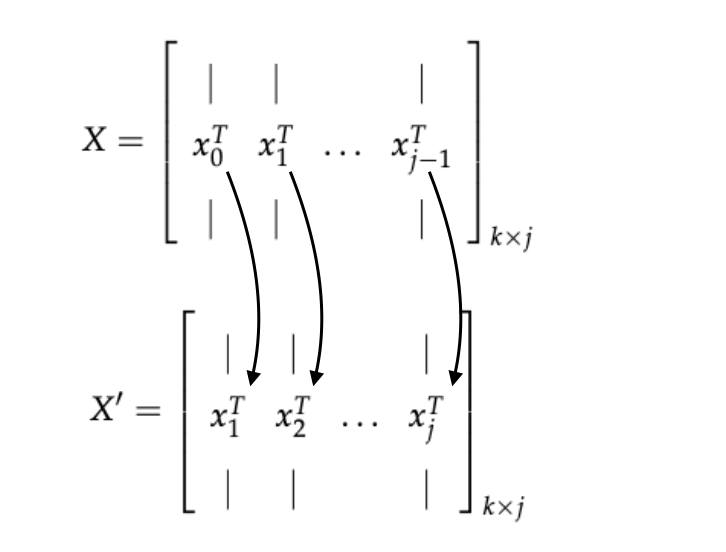
\includegraphics[width=0.65\textwidth]{X to X'.png}
    \caption{$X$ to $X'$}
\end{figure}

Where %Ask Tim
\begin{equation}
\vec{x}_{0}\longrightarrow \vec{x}_{1},....,\vec{x}_{j-1}\longrightarrow \vec{x}_{j} \\
%\lbrack x_{i}] &\longrightarrow &A_{i}[x_{i+1}],i=0,1,..m????? \\
\end{equation}

After performing the algorithm for the computation we would like to minimize
the error $\parallel X'-AX \parallel_{F}$ where $F$ is the
Frobenius norm is given by

\begin{equation}
    \parallel{X\parallel}_{F} = \sqrt{\sum_{j=1}^{n}\sum_{i=1}^{m}X_{ji}^{2}}
\end{equation}

We can solve for A via a Moore-Penrose pseudo-inverse. We can rearrange $%
X^{^{\prime }}=AX$ to solve for $A$ using the Moore-Penrose Pseudo Inverse,
to give $A=X^{^{\prime }}X^{\dagger }$ where $X^{\dagger }$ is the pseudo-inverse of $X$. $X$ is a $k\times j$ matrix and $X^{^{\prime }}$ is $%
k\times j$ matrix. Hence the $X^{\dagger }$ is a $j\times k$ yielding $A$
to be a $k\times k$ square matrix. Examples of the Moore-Penrose pseudo-inverse will be given below.
\begin{equation}
X^{\dagger}=
    \begin{cases}
        X^{T}(XX^{T})^{-1} & \text{if }X\text{ \small{is an onto linear map of independent rows}} \\
        (XX^{T})^{-1}X^{T} & \text{if }X\text{ \small{is a 1-1 linear map of independent columns}}
    \end{cases}
\end{equation}

For $X$ and $X^{^{\prime }}$, we perform the Compact Singular Value Decomposition upon $X$. The compact form of SVD is given by there exist
matrices $U, \Sigma, V$ of type $k\times r,r\times r,r\times k$
respectively, such that $X=$ $U\Sigma V^{T}$and $UU^{T}=VV^{T}=I,$ \ where $r=\min (k,j).$ That is,
\begin{equation}
    \begin{aligned}
        X&= U_{k\times k}\Sigma _{k\times j}V_{k\times j}^{T}\text{ for regular SVD} \phantom{33}\\
        X& = U_{k\times r}\Sigma _{r\times r}V_{r\times k}\text{ for compact numerical SVD}
    \end{aligned}
\end{equation}

The eigenvalues of $V$ are from $AA^{T}$, the eigenvalues of $U$ are from $%
AA^{T}$  
Solving For $A$ Using the SVD of $X$ yields
\begin{equation}
A =X'_{k\times j}(U_{k\times r}\Sigma_{r\times r} V^{T}_{r\times j})^{-1} =X'_{k\times j}V_{j\times r}\Sigma^{-1}_{r\times r}U^{T}_{r\times k}
\end{equation}

One way of doing SVD is by using the Polar Decomposition of a square matrix. Given a square $k\times k$ matrix $A$, $A$ can be written as $A=R_{1}S$, where $R_{1}$ is an orthogonal matrix and $S$ is a symmetric matrix. A symmetric matrix can be diagonalized hence
\begin{equation}
    \begin{aligned}
        A &\;= R_{1}S \\
        &=R_{1}(R_{2}DR_{2}^{T}) \\
        &=(R_{1}R_{2})DR_{2}^{T} \\
    \end{aligned}
\end{equation}
Where
\begin{equation}
    \begin{cases}
        U=(R_{1}R_{2})\\
        \Sigma =D\\
        V=R_{2}
    \end{cases}
\end{equation}

Hence we get an SVD of $A$ from a polar Decomposition. It is more efficient to project our Matrix $A$ onto the $r\times r$ subspace of the $k\times k$ subspace so the calculations are less taxing.
We do do this by rearranging our matrix $A=X^{^{\prime }}V\Sigma ^{-1}U^{T}$
and then orthogonally projecting onto the $r\times r$ subspace.
\begin{equation}
    \begin{aligned}
    A&\;=X^{^{\prime }}V\Sigma ^{-1}U^{T} \\
    \Longrightarrow AU&=X^{^{\prime }}V\Sigma ^{-1} \\
    \Longrightarrow U^{T}AU&=U^{T}X^{^{\prime }}V\Sigma ^{-1}
    \end{aligned}
\end{equation}

The $U^{T}AU$ is the orthogonal projection of $A$ onto the $r\times r$
subspace. \ label $U^{T}AU=\widetilde{A\text{.}}$ \ We check the Dimensions
of $U^{T}AU$. \ The matrix $U^{T}AU$ is given by matrices $U^{T},A,U$ of
type $r\times k,k\times k,k\times r$ respectively, hence $\widetilde{A}$ is
of type $r\times r.$ \ The matrix $\widetilde{A}$ defines a lower rank
linear model of the form  $\widetilde{A}\widetilde{x_{l}}=\widetilde{x}_{l+1}
$. \ Where the vectors $\widetilde{x_{l}}$ are of type $r\times 1$. \ We can
reconstruct the the original data by using the $U$ matrix given by $x_{l}=U%
\widetilde{x}_{l+1}$. \ 

We now compute the eigenvalues and eigenvectors of $\widetilde{A}$ , which
will give an eigenvector basis. \ Let $W$ be the eigenvector matrix
associated to the eigenvectors of $\widetilde{A}$. \ We can then reconstruct
the eigendecomposition of $A$ from $W$. \ Where we are given that $%
\widetilde{A}W=W\Lambda $ \ where $\Lambda $ is the matrix of eigenvalues. Hence 
\begin{equation}
    \begin{aligned}
    &\phantom{3333i} U^{T}AU=W\Lambda W^{T} \\
    &\Longrightarrow A=UW\Lambda W^{T}U^{T} \\
    &\Longrightarrow A=(UW)\Lambda (UW)^{T} \\
    &\Longrightarrow AU=X^{^{\prime }}V\Sigma ^{-1}=UW\Lambda W^{T} \\
    &\Longrightarrow AUW=X^{^{\prime }}V\Sigma ^{-1}W:=\Phi  \\
    &\Longrightarrow A_{k\times k}U_{k\times r}W_{r\times r}:=\Phi _{_{k\times r}}
    \end{aligned}
\end{equation}

Notice that $A_{k\times k}U_{k\times r}W_{r\times r}:=\Phi _{_{k\times r}}$
is the alternate form of the SVD. \ Also note that if  $\Phi _{1}=UW$ then \ 
$\Phi _{1}$ will converge to $\Phi $ if $X$ and $X^{^{\prime }}$ have the
same column space. \ $\Phi _{1}=UW$ are known as the projected DMD modes. \
The modes in $X^{^{\prime }}V\Sigma ^{-1}W:=\Phi $ are termed exact modes.

\section{Koopman Spectral Theory}

Notice that $A_{k\times k}U_{k\times r}W_{r\times r}:=\Phi _{_{k\times r}}$
and that if $\Phi _{1}=UW$ then \ $\Phi _{1}$ will converge to $\Phi $
if $X$ and $X^{^{\prime }}$ have the same column space. \ $\Phi _{1}=UW$ are
note as the projected DMD modes. \ The modes in $X^{^{\prime }}V\Sigma
^{-1}W:=\Phi $ are termed exact modes. 

Given a system $\frac{dx}{dt}=f(x,t)$ and the associated system $\frac{dx}{dt%
}=Bx$, One solves this system by using the exponential matrix, that is $%
x(t)=c_{1}v_{1}e^{\lambda _{1}t}+\ldots +c_{n}v_{n}e^{\lambda _{n}t}$ where
for $i=1..n$, $c_{i}$ are constants, $v_{i}$ are eigenvectors and $\lambda
_{i}$ are the eigenvalues. Similarly for our system, $x(t)=\sum \limits_{k=1}^{r}\phi _{k}\exp (\omega_{k}t)b_{k}$ which in compact matrix
notation becomes $x(t)=\Phi \exp (\Omega t)\mathbf{b}_{k}$, where $\Omega
=diag(\omega)$ is a diagonal matrix with eigenvalues $w_{k}=\ln (\lambda
_{k})/\Delta t$ where we use the $\ln (\lambda _{k})$ to smooth out large
eigenvalues. The eigenvectors of \ $\Phi $ are given by $\phi _{k}$ and $b_{k}$ can be solved by evaluating $x(0)=x_{1}$ and $\mathbf{b}=\Phi
^{\dagger}x_{1}$, where $\Phi ^{\dagger}$ is the Moore Penrose Pseudo Inverse. $x(t)=\sum\limits_{k=1}^{r}\phi _{k}\exp (\omega_{k}t)b_{k}$ is interpreted as a least square fit in the sense of the two norms given by $\parallel x_{k+1}-Bx_{k}\parallel _{2}$ and iterating $\frac{dx}{dt}=Bx$ gives $x_{k+1}=Bx_{k}.$ 

If a low dimension representation exists then as iterations are done the singular values in the matrix $\Sigma $ will appear and the $\ast \ast $ below will converge to zero where $\sum\limits_{k=1}^{r}\sigma_{k}^{2}=tr(A^{T}A).$

\begin{equation}
    \Sigma =%
    \begin{bmatrix}
    \sigma _{1} &  &  &  &  \\ 
    & \sigma _{2} &  &  &  \\ 
    &  & \ddots &  &  \\ 
    &  &  & \ddots &  \\ 
    &  &  &  & \sigma _{r} \\ 
    \ast  & \ast  & \ast  & \ast  & \ast  \\ 
    \ast  & \ast  & \ast  & \ast  & \ast 
    \end{bmatrix}
\end{equation}

Hence this is why it is considered a dimension-reducing algorithm.   

\subsection{Application in DMD} 

For $g:%
%TCIMACRO{\U{2102} }%
%BeginExpansion
\mathbb{C}
%EndExpansion
^{n}\longrightarrow 
%TCIMACRO{\U{2102} }%
%BeginExpansion
\mathbb{C}
%EndExpansion
$, $g$ is a function that takes our snapshot frame and spits out a number,
we think of this function as a measurement. \ We will use this in
conjunction with a flow map. \ Define a flow map by

\begin{equation}
    F_{t}(x_{0}):=x(t+t_{0})=x(t_{0})+\int\limits_{t_{0}}^{t+t_{0}}f(x,\tau
    )d\tau
\end{equation}

This comes from integrating the equation $\frac{dx}{dt}=f(x,t)$. \ We can
now iterate the flow map to get

\begin{equation}
    x_{k+1}=F_{t}(x_{k})=x(t_{0})+\int\limits_{t_{0}}^{t+t_{0}}f(x_{k},\tau
    )d\tau
\end{equation}

We now introduce the Koopman operator $K.$ \ The Koopman operator acts on
functions by a composition map defined by

\begin{equation}
    Kg=g\circ f
\end{equation}

We apply this to our flow map to get 

\begin{equation}
    \begin{aligned}
        Kg(x_{k}) &=g\circ F_{t}(x_{k}) \\
        &=g(x_{k+1})
    \end{aligned}
\end{equation}

Hence we see that the Koopman operator advances measurements from $%
g(x_{k})$ to $g(x_{k+1})$. \ We have an analogous setup to that Of the DMD
below since the Koopman operator advances measurements
\begin{figure}
    \centering
    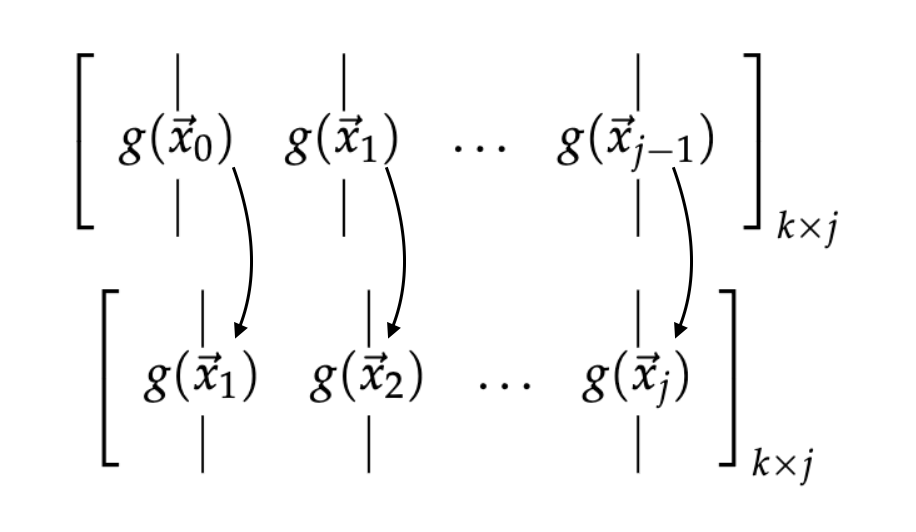
\includegraphics[width=0.6\textwidth]{g(X) to g(X').png}
    \caption{Koopman Advanced Measurements}
    \label{kooppic}
\end{figure}

\ 

Koopman looked at Hamiltonian flows that were measure preserving, hence
unitary in nature. \ 

The Koopman operator lives in the space known as the Hilbert space. \ The
Hilbert space is equipped with a norm called the $L_{2}$ norm, given by $%
\parallel f\parallel _{L_{2}}=\int \mid f\mid ^{2} < \infty $. 

One can look at the eigenvalues of the Koopman operator analogous to looking at
the eigenvalues of matrices. \ With regards to Matrices and eigenvalues $Ax=lx$
for an eigenvalue $l$ and an eigenvector $x$. \ Let $\phi $ be an
eigenfunction of the Koopman operator then $K\phi =\lambda \phi $, where $%
\lambda $ is the associated eigenvalue. \ We give an example of this.

\begin{equation}
    \begin{aligned}
        \text{let }g(x) &=(\log (x))^{c} \\
        \text{let }f(x) &=x^{p} \\
        Kg(x) &=(g\circ f)(x) \\
        &=(\log (x^{p}))^{c} \\
        &=(p\log (x))^{c} \\
        &=p^{c}(\log (x))^{c} \\
        \lambda  &=p^{c}
    \end{aligned}
\end{equation}

Instead of $g$ being a single function that the Koopman operator acts on, we
can consider a vector of measurement functions given by $(g_{1}(%
\vec{x_{i}}),.......,g_{k}(\vec{x_{i}}))^{T}.$ We can write 
\begin{equation}
\vec{g}(x)=\sum\limits_{k=1}^{\infty }\phi _{k}v_{k}
\end{equation}

Where we use the $L_{2}$ norm to find the $v_{k}$ given by%
\begin{equation}
v_{k}=%
\begin{bmatrix}
\left\langle \phi _{k},g_{1}\right\rangle _{L_{2}} \\ 
\left\langle \phi _{k},g_{2}\right\rangle _{L_{2}} \\ 
.. \\ 
.. \\
.. \\ 
\left\langle \phi _{k},g_{k}\right\rangle _{L_{2}}%
\end{bmatrix}%
\end{equation}

Instead of having a finite vector basis as we would have in the regular DMD,
we now have an infinite dimensional space spanned by the eigenvectors $%
\{\phi _{k}\}$. The Koopman operator can act on the vector-valued function $\vec{g%
}(x)$ in a linear way. 
\begin{equation}
    \begin{aligned}
    K\vec{g}(x) &=K\sum\limits_{k=1}^{\infty }\phi _{k}v_{k} \\
    &=\sum\limits_{k=1}^{\infty }K\phi _{k}v_{k} \\
    &=\sum\limits_{k=1}^{\infty }\lambda _{k}\phi _{k}v_{k}
    \end{aligned}
\end{equation}

Where we have expanded $\vec{g}(x)$ using the eigenfunction basis. If $g$ is chosen well it can simplify calculations, we give a heuristic view of this via figure ($\ref{fig:koop}$).

\begin{figure}[H]
    \centering
    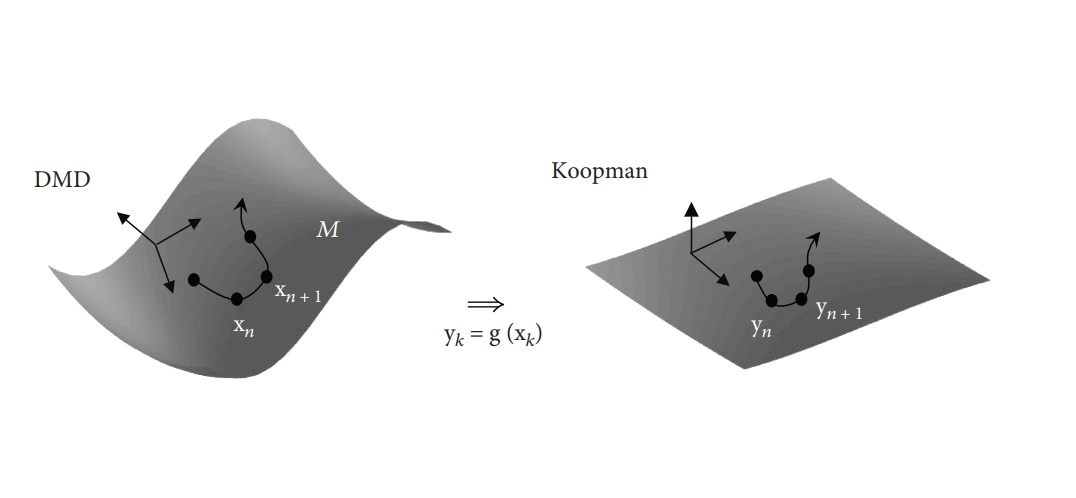
\includegraphics[width=1\textwidth]{koop.jpg}
    \caption{Visual representation of the Koopman operator restricted to a finite-dimensional invariant subspace spanned by Eigen functions} \label{fig:koop}
\end{figure}
\noindent

If $g$ is chosen well it can take a flow on a nonlinear manifold to a
more linearized version in which calculations can become more manageable. Given the above construction, we can now perform DMD in Hilbert space
analogous to DMD in a vector space with the euclidean norm.

\begin{eqnarray*}
Y &=&%
\begin{bmatrix}
.. & .. & .. & .. & .. \\ 
.. & .. & .. & .. & .. \\ 
\vec{g}([x_{0}]^{T}) & \vec{g}([x_{1}]^{T}) & .. & ..
& \vec{g}([x_{j-1}]^{T}) \\ 
| & | & .. & .. & | \\
| & | & .. & .. & |%
\end{bmatrix}
\\
Y^{^{\prime }} &=&%
\begin{bmatrix}
| & | & .. & .. & \phantom{-}| \\ 
\downarrow  & \downarrow  & .. & .. & \phantom{p}\downarrow  \\ 
\vec{g}([x_{1}]^{T}) & \vec{g}([x_{2}]^{T}) & .. & ..
& \phantom{i}\vec{g}([x_{j}]^{T}) \\ 
.. & .. & .. & .. & \phantom{-}.. \\ 
.. & .. & .. & .. & \phantom{-}..%
\end{bmatrix}%
\end{eqnarray*}

We now perform SVD on $Y$ and follow the algorithm previously defined in the DMD.

If $\phi _{k}\in span$ $(g_{1}(\vec{x_{i}}),.......,g_{p}(%
\vec{x_{i}}))^{T}$ then $\phi _{k}=a_{1}g_{1}+.........+a_{p}g_{p}$ and $p$ is not necessarily equal to $k$, the $a_{i}$ are constants in the field

\begin{equation}
    \begin{aligned}
        K\phi _{k} &=\lambda _{k}\phi _{k} \\
        &=\lambda _{k}(a_{1}g_{1}+.........+a_{p}g_{p}) \\
        &=\lambda _{k}a_{1}g_{1}+.........+\lambda _{k}a_{p}g_{p}
    \end{aligned}
\end{equation}

Hence K becomes a linear operator. For if  $[a_{1},........,a_{p}]^{T}\in Range(Y)$ then $a=[a_{1},........,a_{p}]^{T}$ is a left eigenvector of $A_{Y}=Y^{\prime}Y^{\dagger}$ and $\vec{a}^{T}A_{Y}=\lambda _{k}\vec{a}^{T}$ We now apply the DMD to get

\begin{equation}
    \begin{aligned}
        \Phi _{Y}:&=Y^{^{\prime }}V\Sigma ^{-1}W \\
        y(t) &=\Phi _{Y}\exp (\Omega t)\mathbf{b} \\
        \mathbf{b} &=\Phi _{Y}^{\dagger}y_{1}
    \end{aligned}
\end{equation}

We now transform back from measured observables to the DMD state space, the
vector space is given by

\begin{equation}
    \begin{aligned}
    y_{k}(x)=\vec{g}(x_{k})\Longrightarrow x_{k}=\vec{g}%
    ^{-1}(y_{k})
    \end{aligned}
\end{equation}
The inversion of $\vec{g}$ can be difficult if not chosen well.

The projected low dimensional solution in Hilbert space of the
Koopman DMD is analogous to the DMD on a finite-dimensional vector space from the relation $\phi _{k}\in span$ $(g_{1}(\vec{x_{i}}%
),.......,g_{p}(\vec{x_{i}}))$ . It is best to make sure we
pick out the dominant(leading) eigenfunctions based on the
(leading)eigenvalue. The relation between DMD and the Koopman DMD is
analogous to a Fourier transform which takes a system from state space to
phase space. Here the state space is the finite-dimensional vector space
in DMD and the Phase space is in the Hilbert Space. One can modify the
Koopman operator and apply to that of Partial Differential Equation (PDE). The Koopman DMD and DMD approximation produce a least squares fit the data of the dynamical
system which approximates the flow map of the system. When the Koopman
operator is chosen well it can potentially linearize the space, hence making the system potentially easier to solve. Dynamics can change when parameters change in the PDE, the dynamics can undergo bifurcation. When the Bifurcation happens the Koopman operators will have to be altered in
conjunction with the bifurcation. We will see in the upcoming data section
that DMD will be applied, DMD has a hard time seeing subtle in-variances
which exist in the system, such as helix style rotations or what is
considered a U(1) gauge and say laminar flow. Invariances undermine the
ability to compute lower dimensional systems since one has to mod out
the specific invariance. To know these invariances one needs to know the
dynamics of the system. This is analogous to if one has a group action on
a manifold, the manifold structure is recovered by modding out the group
action. The DMD algorithm can be regarded as an application of a flow on the
manifold of fixed rank matrices which is then projected onto a lower
dimensional manifold. The vector field of the flow of the original
system is projected onto the tangent space of the lower dimensional
manifold. Here the geometry of fixed rank matrices can be studied. 

The predictive power of DMD is not expansive and needs to be improved. One
way of improving the predictive power is to add an existing known control
into the system, by which the control is governed. The system would be
in the form of $X^{\prime }=AX+CY$ where $C$ is a matrix, possibly of
functions, which steers the system. $Y$ is a set of new snapshots
similar to $X$ though is considered a control snapshot. One would then get 
$(X^{^{\prime }}-CY)V\Sigma ^{-1}U^{T}=A.$

\section{APPLICATION TO PDEs}

We look at Burger's equation

\begin{equation}
u_{t}+u_{x}u-\varepsilon u_{xx}=0,\varepsilon >0
\end{equation}
The existence of the diffusion term is known to regularize the PDE.
We transform the PDE using
\begin{equation}
u=-2\varepsilon v_{x}/v
\end{equation}
the PDE transforms as
\begin{equation}
v_{t}=-\varepsilon v_{xx}
\end{equation}
We then us the Fourier Transform on the above PDE.
the Fourier Transform is given by

\begin{equation}
\widehat{v}(k,t)=\int_{-\infty }^{\infty }v(x,t)e^{-ikx}dx
\end{equation}

We use the property $F(\frac{d}{dx}(f(x))=ik\widehat{f}(k)$ and $F(\frac{%
d^{n}}{(dx)^{n}}(f(x))=(ik)^{n}\widehat{f}(k)$ and apply this to $%
v_{t}=-\varepsilon v_{xx}$

\begin{equation}
    \begin{aligned}
        \widehat{v}_{t} &=-\varepsilon k^{2}\widehat{v} \\
        \widehat{v} &=\widehat{v_{0}}\exp (-\varepsilon k^{2}t)
    \end{aligned}
\end{equation}

Using $u=-2\varepsilon v_{x}/v$ and $\widehat{v}=\widehat{v_{0}}\exp
(-\varepsilon k^{2}t)$ one can construct a Koopman Operator via composition
of the Fourier transform with $u=-2\varepsilon v_{x}/v$
Hence one gets

\begin{equation}
v(x,t)=exp\left(-\dfrac{\int_{-\infty}^{x}u(\alpha,t)d\alpha}{2\epsilon}\right)
\end{equation}
We verify this works by checking $u=-2\varepsilon v_{x}/v$

\begin{equation}
v_{x}(x,t)=\frac{d}{dx}\left( -\frac{\int_{-\infty }^{x}u(\alpha
,t)d\alpha}{2\varepsilon}\right) \exp \left( -\frac{\int_{-\infty}^{x}u(\alpha,t)d\alpha }{2\varepsilon }\right) 
\end{equation}
Using the fundamental theorem of calculus on $\frac{\int_{-\infty
}^{x}u(\alpha,t)d\alpha}{2\varepsilon}$ we get

\begin{equation}
\begin{aligned}
        v_{x}(x,t) &=\frac{u(x,t)}{-2\varepsilon }v(x,t) \\
        u(x,t) &=(-2\varepsilon)\frac{v_{x}(x,t)}{v(x,t)}
    \end{aligned}
\end{equation}
And this verifies our function works. We define our Koopman Operator $g$ by
\begin{equation}
g(u)=\widehat{v}
\end{equation}


\chapter{Interpretation}
DMD decomposes complex flows into their fundamental spectral components which correspond to spatial and temporal properties that characterize the behaviour of the flow. Thus in order to extract useful information from the DMD analysis an understanding of the computed eigenvalues and eigenvectors of the best fit DMD operator A is essential. Detailed interpretation of the eigenvalues and eigenvectors of an equation \eqref{dfeq} will be provided in this section.

\begin{equation}\label{dfeq}
    x(t)={\Phi}exp(\Omega{t}){\textbf{b}}
\end{equation}

\section{Interpretation of Eigenvectors}
The eigenvectors $\Phi$ of the dynamic mode decomposition also referred to as the DMD modes represent the spatial properties of the system or data field being analyzed. Each entry of a vector-valued mode corresponds to a spatial location of the data field and can be used to identify both local and global features such as mixing, symmetry, and long-time behaviour. Each eigenvector is scaled by an amplitude \textbf{b} which is also determined during the analysis by DMD and is used to determine each mode's influence. The more dominant the mode the more it is represented in the decomposition of the data. This helps to allow for the selection of the relevant modes to be made. 

\section{Interpretation of Eigenvalues}
The eigenvalues $\lambda$ of a mode allow us to determine the temporal development or dynamical behaviour of said mode. These eigenvalues can be plotted on a complex-valued unitary circle which represents stable or stationary flow structures, their position on the circle presents information regarding frequency and growth rate. The eigenvalues found from the analysis with DMD are discrete eigenvalues, for better interpretation they can be converted into continuous time eigenvalues. The transformation from discrete to continuous time eigenvalues is done using equation \eqref{de>cte} where the $\Delta{t}$ is the time between snapshots. 

\begin{equation}\label{de>cte}
    \Omega=\frac{ln(\lambda)}{\Delta{t}}
\end{equation}

Eigenvalues can be sorted into three categories based on their location in the complex unitary circle. When considering discrete eigenvalues, if the eigenvalue corresponds to a point within the unit circle, which will decay and vanish over time. If the point can be found on the unit circle then it will oscillate over time. Finally, if the point appears outside the unit circle that means it will grow and diverge over time. After the transformation to continuous time eigenvalues, we see that decaying modes occur when Re($\Omega$) < 0, oscillating modes occur when Re($\Omega$) = 0, and growing modes occur when Re($\Omega$) > 0. A summary of the temporal behaviour of discrete and continuous time eigenvalues is presented in Table (\ref{tab:tempsum}). 

\begin{table}[H] 
\caption{Temporal Behaviour Summary} \label{tab:tempsum}
\centering
\begin{adjustbox}{width=1\textwidth}
\small
\begin{tabular}{|c|c|c|}
\hline
{\textbf{Discrete Eigenvalue}} & {\textbf{Continuous time Eigenvalue}} & {\textbf{Temporal Evolution}} \\ \hline
Inside the unit circle        & Re($\Omega$)<0              & Decaying  \\ \hline
On the unit circle            & Re($\Omega$)=0              & Oscillating   \\ \hline
Outside the unit circle       & Re($\Omega$)>0              & Growing       \\ \hline
\end{tabular}
\end{adjustbox}
\end{table}
\noindent

To show just how beneficial it is to transform the eigenvalues from discrete time to continuous time eigenvalues an example data set was analyzed using DMD. The original and transformed eigenvalues were plotted beside each other for comparison in figure (\ref{fig:comp}). It is clearly much easier to differentiate between the different types of temporal behaviour using the continuous-time eigenvalues.

\begin{figure}[H]
    \centering
    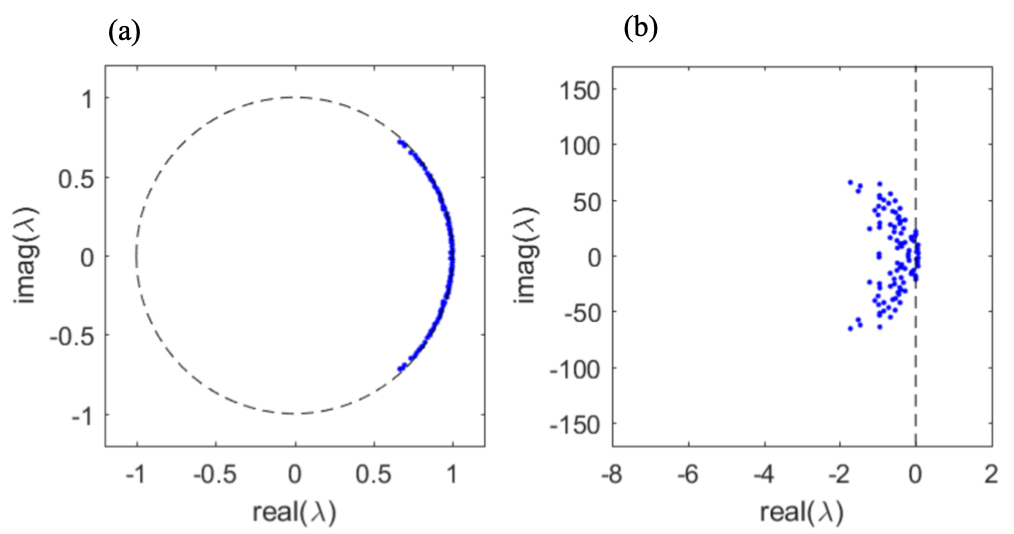
\includegraphics[width=0.9\textwidth]{Application pics/MA680 Dis to Con (Ep).png}
    \caption{Spectrum Plot Comparison of (a) discrete versus (b) continuous time eigenvalues} \label{fig:comp}
\end{figure}
\noindent

A visual representation of each type of temporal evolution is depicted in figure (\ref{fig:modeEv}). The red line represents a decaying mode, the green line represents a growing mode and the blue line represents an oscillating mode. 

\begin{figure}[H]
    \centering
    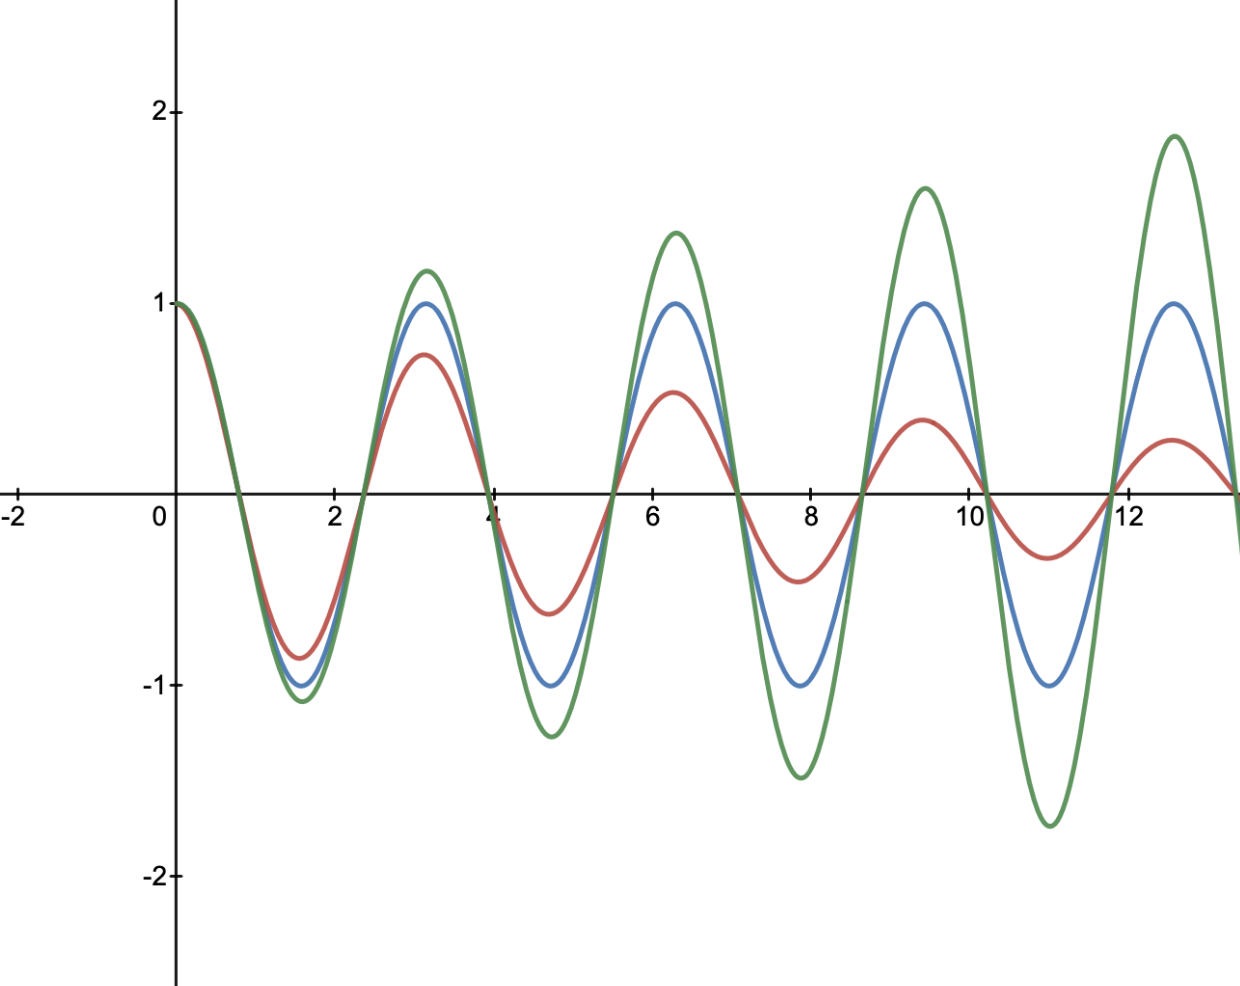
\includegraphics[width=0.5\textwidth]{mode evolution.png}
    \caption{Time Evolution of Each Type of Mode} \label{fig:modeEv}
\end{figure}
\noindent
\chapter{Application}
The DMD technique can be applied to a multitude of areas, the two we looked at were its application to modelling the spread of infectious disease, and to the development of financial trading strategies.

\section{Modeling infectious disease spread}
Outbreaks of infectious diseases are the cause of death for millions of people worldwide each year. Stopping the spread of infectious diseases is one of the most important objectives of global health. Unfortunately due to its complexity and a lack of a single set of physics-based equations governing it, modelling its spread can be challenging. One such solution to this problem is dynamic mode decomposition, as the equation-free nature of DMD makes it easier to analyze infectious disease data. 

An example of DMD applied to infectious disease data is described in \cite{Epidemiology}, it was applied to Google’s Flu Trends tool, which used aggregated Google search data and historical flu data to construct a method for determining the state of flu activity. The collection of data consists of a two-dimensional array with the location axis showing state, city, and health and human services region, while the time axis shows seven-day advancements. A visualization of the flu trend data for each of the 50 states in America is shown in figure (\ref{fig:GFTData}). Note that the y-axis is the number of standard deviations from the mean and 0 represents the historic baseline level of influenza activity for its corresponding region. 

\begin{figure}[H]
    \centering
    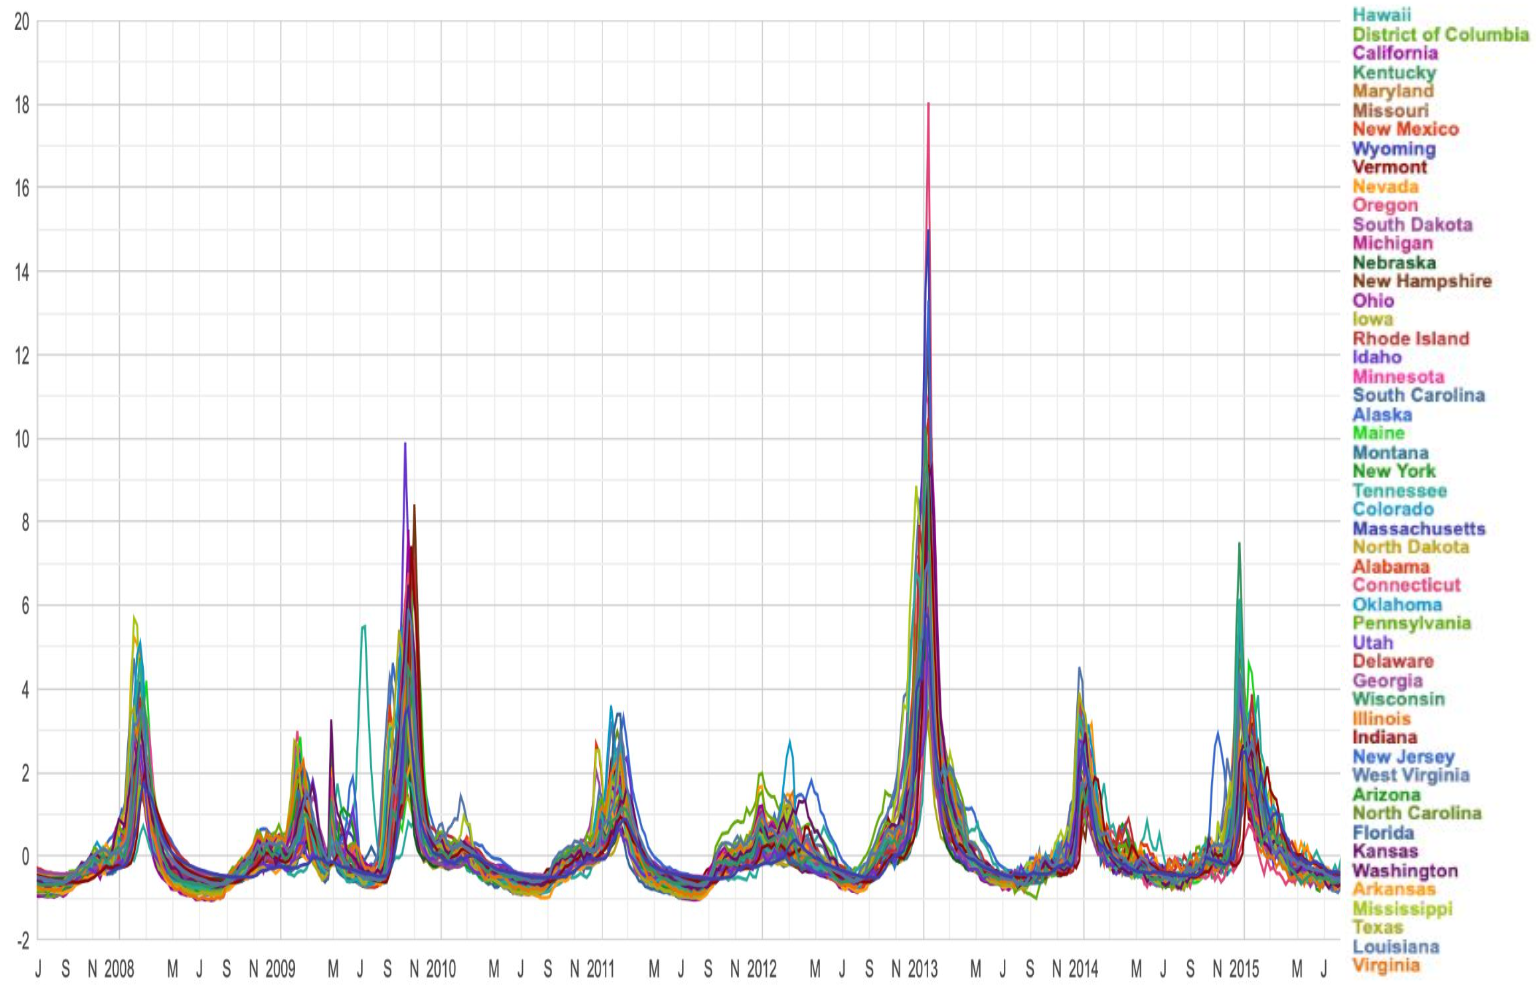
\includegraphics[width=1.1\textwidth]{Application pics/GFT.png}
    \caption{Google Flu Trends Data for United States \cite{GFT}} \label{fig:GFTData}
\end{figure}
\noindent

Vectors can be constructed from the data collected at different spatial locations in order to represent the evolution of state snapshots over time. Spatial and temporal patterns extracted from the dataset are represented by the collection of eigenvalues and their respective dynamic modes of decomposition. 

The dynamic modes or eigenvectors give two critical insights into the disease system being modelled. The first is the magnitude of the mode, which allows us to quantify the spatial location’s participation in that mode. The second is the angle between the real and imaginary components of the mode, which indicates the spatial location's phase of oscillation compared to the other locations in the analysis. 

The eigenvalues are used as described above to determine the temporal nature of each dynamic mode as time progresses. Because it can be challenging to interpret the oscillatory frequency for a given $\Delta{t}$ in the complex plane this paper converted from discrete to continuous time eigenvalues and then to a continuous oscillatory frequency via equation \eqref{fluconv}. Note that the $\Delta$t was 7 days in this case.
\begin{equation}\label{fluconv}
    frequency_{j}=\frac{imag(ln(\lambda_{j})/\Delta{t})}{2\pi}
\end{equation}

\subsection{DMD Output}

The discrete eigenvalues determined from the dynamic mode decomposition are displayed in the following figure (\ref{fig:GFTDEv}). The eigenvalue distribution on the unit circle shows that a large number of eigenvalues fall well inside the unit circle. This means their corresponding dynamic modes are fast decaying and thus do not help to explain the long-term evolution of the disease system.   

\begin{figure}[H]
    \centering
    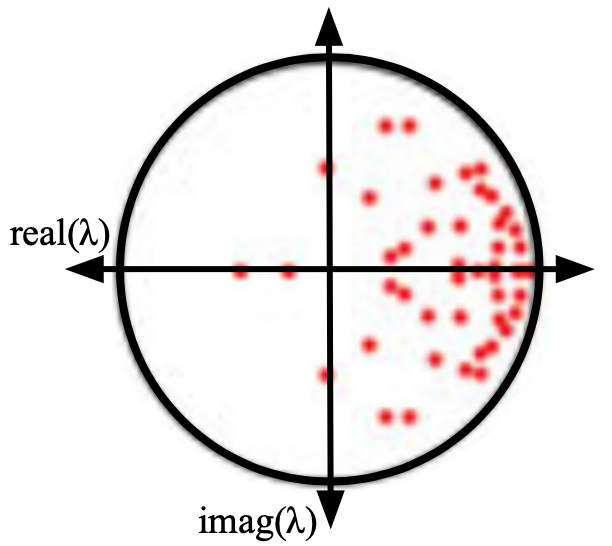
\includegraphics[width=0.35\textwidth]{Application pics/MA680 Ep. eigen.png}
    \caption{Discrete Eigenvalue Spectrum} \label{fig:GFTDEv}
\end{figure}
\noindent

A quantification of the level of dominance of each mode can be made by combining the decay rates of these eigenvalues with the overall magnitude of their corresponding modes and the number of iterative steps in the following relation \eqref{dominance}. The mode selection plot Figure (\ref{fig:msp}) presents a comparison of the dominance of each mode and is used to select the most relevant mode of the long-term behaviour. 
\begin{equation}\label{dominance}
    power =\lambda^{p}_{j}\parallel\phi_{j}\parallel
\end{equation}

\begin{figure}[H]
    \centering
    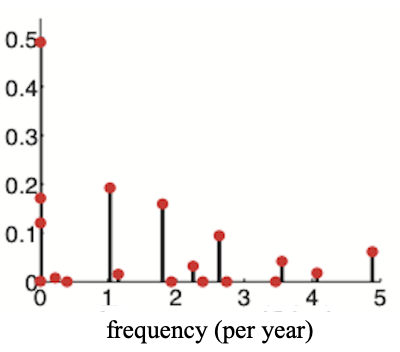
\includegraphics[width=0.4\textwidth]{Application pics/MA680 MSP (Ep).png}
    \caption{Mode Selection Plot} \label{fig:msp}
\end{figure}
\noindent

From the mode selection plot, it is evident that the relevant mode that should be chosen is the one associated with the once-per-year frequency as it is the most dominant. Figure (\ref{fig:map}) is an illustration of how the phase space of the selected dynamic mode can be plotted on a map of the United States, where each element of the dynamic mode represents a location on the map. The phase was plotted on a scale of 0 to 1 with that value indicating the time of year. Due to the fact that the phase value exists on a circle, the values near 0 and 1 are actually close in phase, which makes intuitive sense when thinking about how December is connected to January.

\begin{figure}[H]
    \centering
    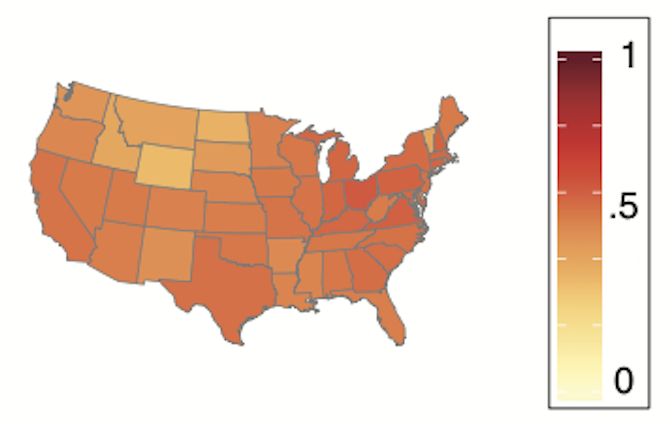
\includegraphics[width=0.75\textwidth]{Application pics/MA680 Map (Ep).png}
    \caption{Yearly Phase Space Plotted on US Map} \label{fig:map}
\end{figure}
\noindent

This phase plot can provide many key insights of high value to public health organizations. For example, it can aid in predicting the best timing to launch the fight against the flu and vaccination campaigns in specific regions. This can be done by observing the change of phase when moving around the map which represents the peak time of flu and the spread of the disease. Furthermore, DMD can be used to identify places with epidemiological connections, which are areas not necessarily geographically connected but share a common phase or time of peak flu activity. This is becoming increasingly relevant as long-distance travel is continuously becoming more commonplace.

\section{Developing Financial Trading Strategies}

At any given time, millions of companies, individuals, institutions, and even governments are trading on financial markets. Regardless of whether the trade is placed by a professional, a novice or an amateur, they all carry some degree of risk, no matter what instrument is traded. In order to be successful in trading and making money, one must balance potential profit against risk. One of the most effective ways to maximize profit is through the use of trading strategies that make use of prior market data. Modern financial investment strategies are becoming increasingly more reliant on algorithmic trading schemes. DMD can be applied to market data to construct financial trading strategies, taking advantage of the growth and decay behaviour of the decomposition. The DMD decomposes stock portfolio data into low-rank features that behave with prescribed time dynamics. Using the least-square fit linear dynamical system, it is possible to predict short-term future states of the system, allowing one to make automated purchases, sales, or hold decisions on investments.

In the paper, \cite{Financial} DMD was applied to a dataset containing stock price quotes over a period between 2005 and 2015 provided by Yahoo! cite finance.yahoo.com. Using the closing prices of the stocks to be analyzed, a data matrix was constructed and organized chronologically with a one-day difference in time ($\Delta{t}$) between data extractions. A diagram illustrating the data matrix being used is shown in figure 1, where each stock can be identified by its stock ticker symbol assigned by the NASDAQ.

\begin{figure}[H]
    \centering
    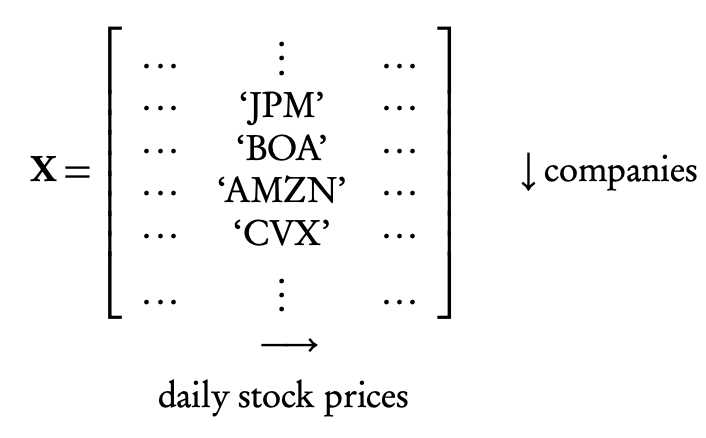
\includegraphics[width=0.7\textwidth]{Application pics/MA680 DMD Financial Matrix X.png}
    \caption{Matrix Representation of Stock Data Provided by Yahoo!} \label{fig:FMatX}
\end{figure}
\noindent

To be able to determine the best combination for predicting the future market the approximate solution for a future time given by $x(t)={\Phi}exp(\Omega{t}){\textbf{b}}$ is instead parameterized by two variables $x(m,l)$. The variable m represents the number of past days of market snapshot data taken, and l represents the number of days in the future predicted, allowing us to control the sampling window and the prediction time frame. Their ranges were set at $1 \leq m \leq 25$ and $1 \leq l \leq 10$, the range for l was chosen as predicting too far into the future decreases the accuracy of the algorithm. The range for m was chosen such that the prior data was sufficiently large enough to capture current trends, but not so long that too much emphasis is placed on the data from the distant past. 

The combinations leading to the optimal predictions are referred to as hot spots, to be considered a hot spot the combination must have a prediction accuracy of 53$\%$ or more, and the average prediction score of this combination and its 8 adjacent cells is at least 53$\%$. Based on empirical observations of the DMD algorithm performance over a 2-year training period from 2005 to 2007, 0.53 was chosen as the optimal prediction threshold. 

\subsection{DMD Output}
Figure (\ref{fig:FSVD}) shows the singular value decomposition for the data matrix X, which is comprised of the portfolio data for 18 companies in the transport and home construction sectors over an 18-day sampling window. Note k represents the number of measurement times and $\sigma_{k}/\sum\sigma_{j}$ represents the $k^{th}$ diagonal element of the diagonal matrix $\Sigma$ found from SVD divided by the sum of the eigenvalues from j to k. The decay of singular values of X can clearly be seen in the image. Since the singular values of sigma decrease sharply to zero we can say that there is a low-rank structure to the data and only 4 dominant modes in the data can be seen. These represent the modes with the maximal variance and are indicated by the colour change. The first mode represents the average price across the sampling window of the 18 companies, and the other 3 modes represent the weightings across the 18 companies. This reveals that the data may be appropriately represented as rank r = 4 allowing for a low-rank truncation to be performed.  

\begin{figure}[H]
    \centering
    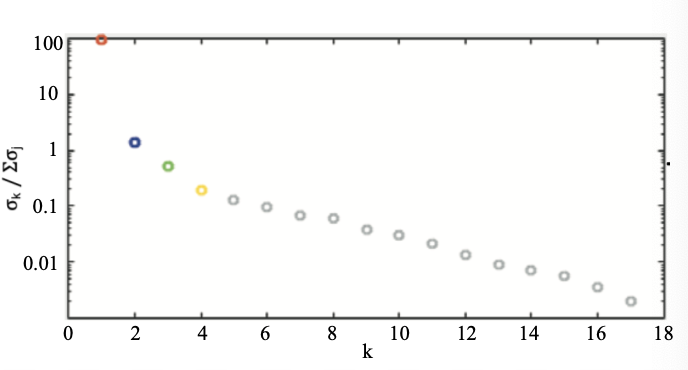
\includegraphics[width=0.8\textwidth]{Application pics/MA680 (F) SVD.png}
    \caption{Singular Values of Data Matrix X on Log Scale} \label{fig:FSVD}
\end{figure}
\noindent

The accompanying spectrum plot of continuous time eigenvalues is shown in (\ref{fig:FEV}). Observe that the eigenvalues appear to cluster along the imaginary axis and many of the eigenvalues are only slightly decaying or growing.  It can be seen that in this case three of the four dominant modes correspond to growth modes. The DMD scheme takes advantage of the largest growth modes to determine the best investment opportunities.   

\begin{figure}[H]
    \centering
    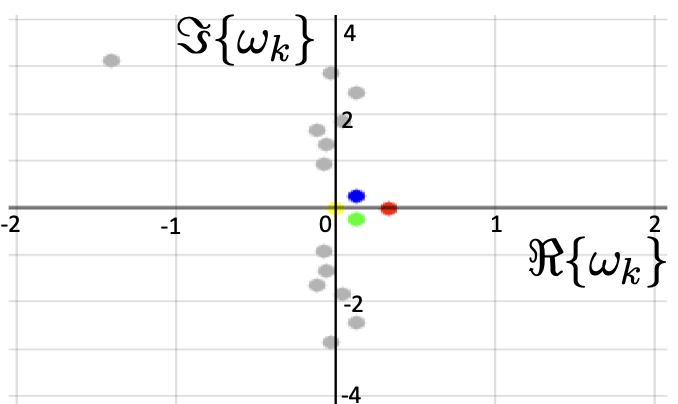
\includegraphics[width=0.6\textwidth]{Application pics/MA680 (F) EV.png}
    \caption{Continuous Time Eigenvalues of Data Matrix X} \label{fig:FEV}
\end{figure}
\noindent

The following figure (\ref{fig:FSR}) shows the success rates achieved using different values for m and l for the DMD algorithm when back-testing, for three portfolios each with 9 companies in either the transport, home construction, or retail sectors over the remaining 8 year period. The optimal values of m and l were determined as explained prior during the 2-year training period and then used to execute trades from 2007 to 2015. The hot spots determined by the dynamic mode decomposition indicated by a star showed a success rate of 53$\%$ or greater over the last 8 years. In other words, 53$\%$ of all the trades executed using that combination was correct and profited. So the best-predicted value for the transport sector occurs when a sampling window of 8 days and a prediction time frame of 4 days are used. The home construction and retail sectors (11,5) and (8,5) provide similar results. 

\begin{figure}[H]
    \centering
    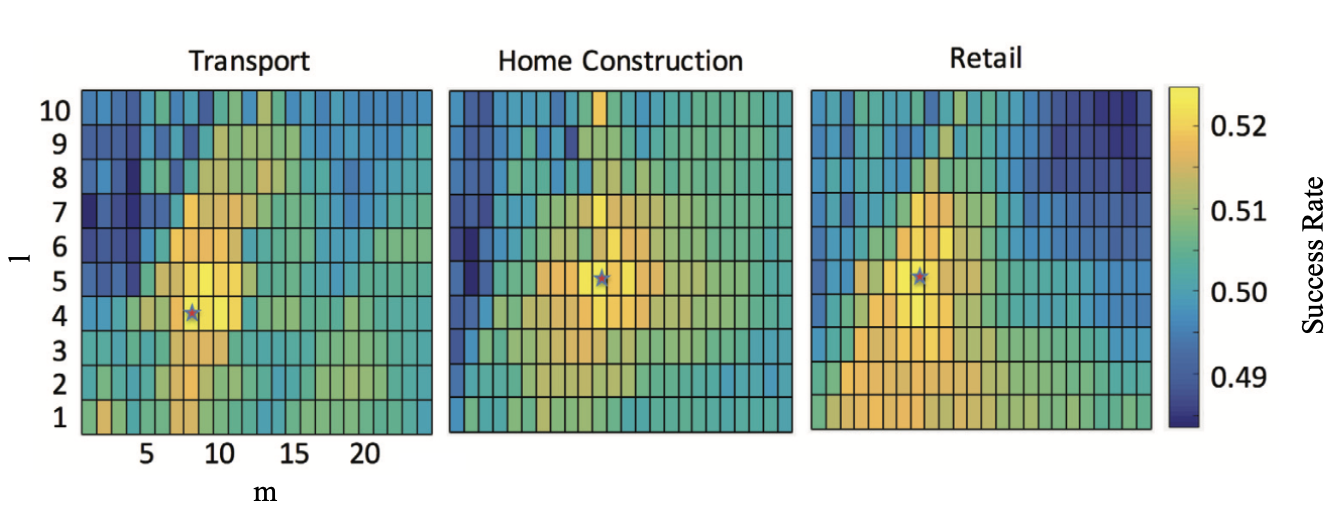
\includegraphics[width=1.1\textwidth]{Application pics/MA680 (F) SR.png}
    \caption{Success Rates of the DMD Algorithm for Transport, Home Construction, and Retail Sectors When Back Testing} \label{fig:FSR}
\end{figure}
\noindent

To assess the DMD trading strategy the potential amount of money earned from the DMD algorithm was computed by theoretically entering a position on every company in the algorithm each day based on the predictions of the algorithm. It is important to note that three assumptions are made, the initial investment capital was $\$$1 million, transaction costs are $\$$8 for each position, and all money is invested evenly across all companies in a given portfolio. The returns for each portfolio over the 8-year period are indicated below (\ref{fig:FSucc}) and are compared to simply holding stock in the S$\&$P500 over the same period. It can be seen that while the transport sector greatly performs the other 2 sectors analyzed with DMD all 3 generate profits well above holding stock in the S$\&$P500 demonstrating the effectiveness of DMD in trading strategies.

\begin{figure}[H]
    \centering
    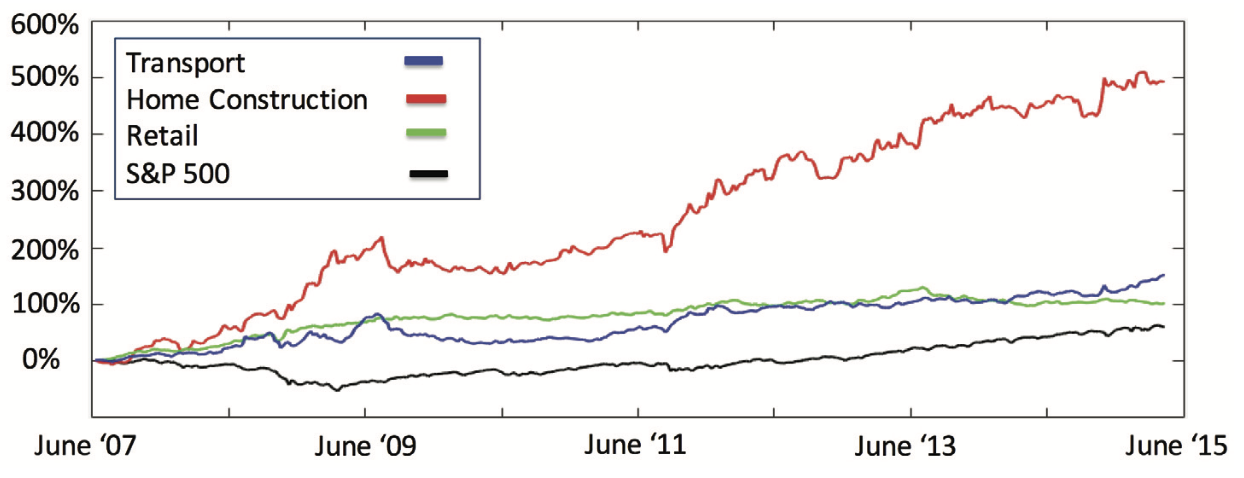
\includegraphics[width=1\textwidth]{Application pics/MA680 (F) Money.png}
    \caption{Trading Success of the DMD Algorithm for the 3 Sectors Compared to Stock in the S$\&$P500} \label{fig:FSucc}
\end{figure}
\noindent

\section{Modelling Weather Systems}

We now apply DMD to weather systems, but we first include a primer on weather systems and supercells.  

Supercell thunderstorms require certain ingredients for them to form. An
unstable Air mass is dictated by warm moist air with warmer air below colder
air, A trigger to start the storms such as a mass of cold air colliding
with the unstable air, shear within the atmosphere and the sun radiating the earth heating the ground creating an unstable environment. Shear is
governed by large changes in wind velocity at different heights above the
earth. Figure (\ref{fig:WS1}) below shows a weather system.

\begin{figure}[H]
    \centering
    \includegraphics[width=0.3\textwidth]{Weather pics/WS1.png}
    \caption{Example Weather system} \label{fig:WS1}
\end{figure}
\noindent

The lines are areas of constant pressure. The white lines are winds. The
kinks in the pressure lines are caused by a cold air mass, as temperature and pressure are related the kinks are caused by sudden changes in temperature and we denote this a frontal boundary. Ahead of the frontal boundary supercells develop which is seen further south in states given by red radar image. Figure (\ref{fig:WS2}) below shows how weather systems resemble a dynamical system.

\begin{figure}[H]
    \centering
    \includegraphics[width=0.3\textwidth]{Weather pics/WS2.png}
    \caption{Weather system Resembling a Dynamical System} \label{fig:WS2}
\end{figure}
\noindent

Low pressure is governed by rising air that rotates counterclockwise, High
pressure is governed by sinking air rotating clockwise. Hence, where the
central low can be thought of as a sink and where the central high can be considered a source. The white lines show where winds converge in both
Figure (\ref{fig:WS1}) and Figure (\ref{fig:WS2}). The converging winds can be thought of as an attractor where the winds converge along the attractor, an area of stability in the dynamical sense. Though the frontal boundary is thermodynamically unstable.

Shear is the main ingredient in rotating updrafts in a supercell. An
idealized updraft of a supercell can be thought of U(1) gauge which
resembles a helix. Figure (\ref{fig:WS3}) below shows the shear.

\begin{figure}[H]
    \centering
    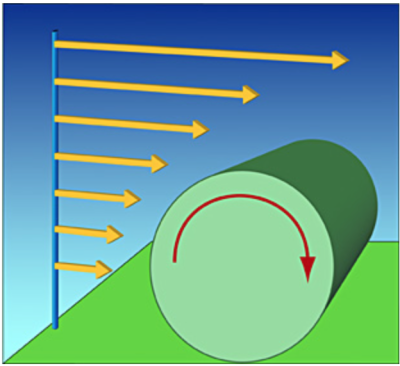
\includegraphics[width=0.5\textwidth]{Weather pics/WS3.png}
    \caption{Visualization of Wind Shear} \label{fig:WS3}
\end{figure}
\noindent

In Figure (\ref{fig:WS3}) the wind speed at higher levels vs lower levels in the atmosphere cause the winds to roll based on fluid dynamics and vorticity. 

In figures (\ref{fig:WS4}) through figure (\ref{fig:WS7}) below we see how the horizontal vorticity gets tilted into a vertical vorticity which is caused by a frontal boundary as a lifting mechanism for the updraft and by the sun radiating earth heating parcels of air which rise as an initial updraft.

\begin{figure}[H]
    \centering
    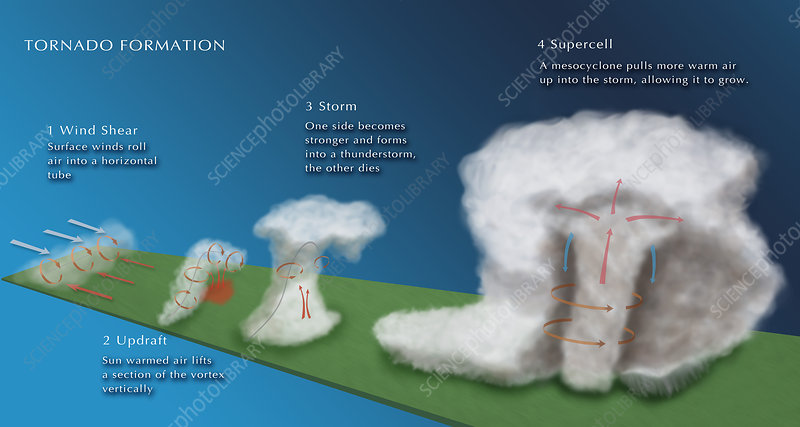
\includegraphics[width=0.9\textwidth]{Weather pics/WS4.jpg}
    \caption{Tornado Formation} \label{fig:WS4}
\end{figure}
\noindent

\begin{figure}[H]
    \centering
    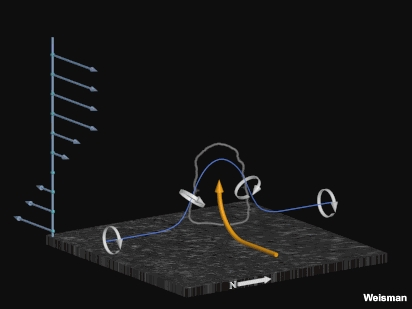
\includegraphics[width=0.6\textwidth]{Weather pics/WS5.jpg}
    \caption{Transition from Horizontal to Vertical Vorticity (I)} \label{fig:WS5}
\end{figure}
\noindent

\begin{figure}[H]
    \centering
    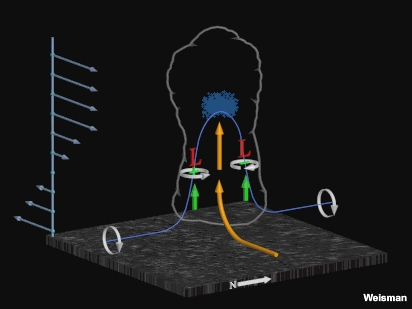
\includegraphics[width=0.6\textwidth]{Weather pics/WS6.jpg}
    \caption{Transition from Horizontal to Vertical Vorticity (II)} \label{fig:WS6}
\end{figure}
\noindent

\begin{figure}[H]
    \centering
    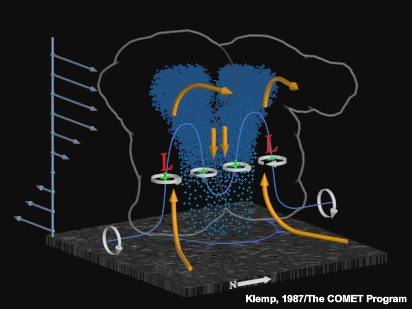
\includegraphics[width=0.6\textwidth]{Weather pics/WS7.jpg}
    \caption{Transition from Horizontal to Vertical Vorticity (III)} \label{fig:WS7}
\end{figure}
\noindent

In Figures (\ref{fig:WS5}) through (\ref{fig:WS7}) as a supercell matures it can create down drafts, which deform the vertical updraft into a sine-like wave which then can make new supercells that either attach to the previous ones or split off to form new ones. Below in figure (\ref{fig:WS8}) is another depiction of an idealized horizontal vorticity which through an updraft and lifting mechanism gets tilted vertically.

\begin{figure}[H]
    \centering
    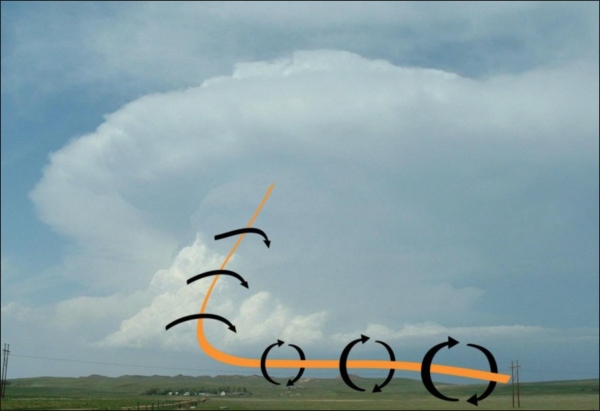
\includegraphics[width=0.8\textwidth]{Weather pics/WS8.png}
    \caption{Real World Example of Vorticity Transition} \label{fig:WS8}
\end{figure}
\noindent

Now with enough background information on weather systems and supercells, we apply DMD to recorded videos of supercells to see how accurate a
lower dimensional representation is of the supercell. We hope it
will capture the dynamics of the system and the rotating updrafts and the
structure.

Figures (\ref{fig:WS9}) and (\ref{fig:WS10}) below are supercell thunder linked by many supercells embedded within, multiple rotating updrafts. Specifically in this photo, two storms are colliding creating a rapid updraft scenario which can be seen in the shelf cloud. A shelf cloud is a very low cloud that sweeps across the above ground and is governed by multiple strong updrafts.

\begin{figure}[H]
    \centering
    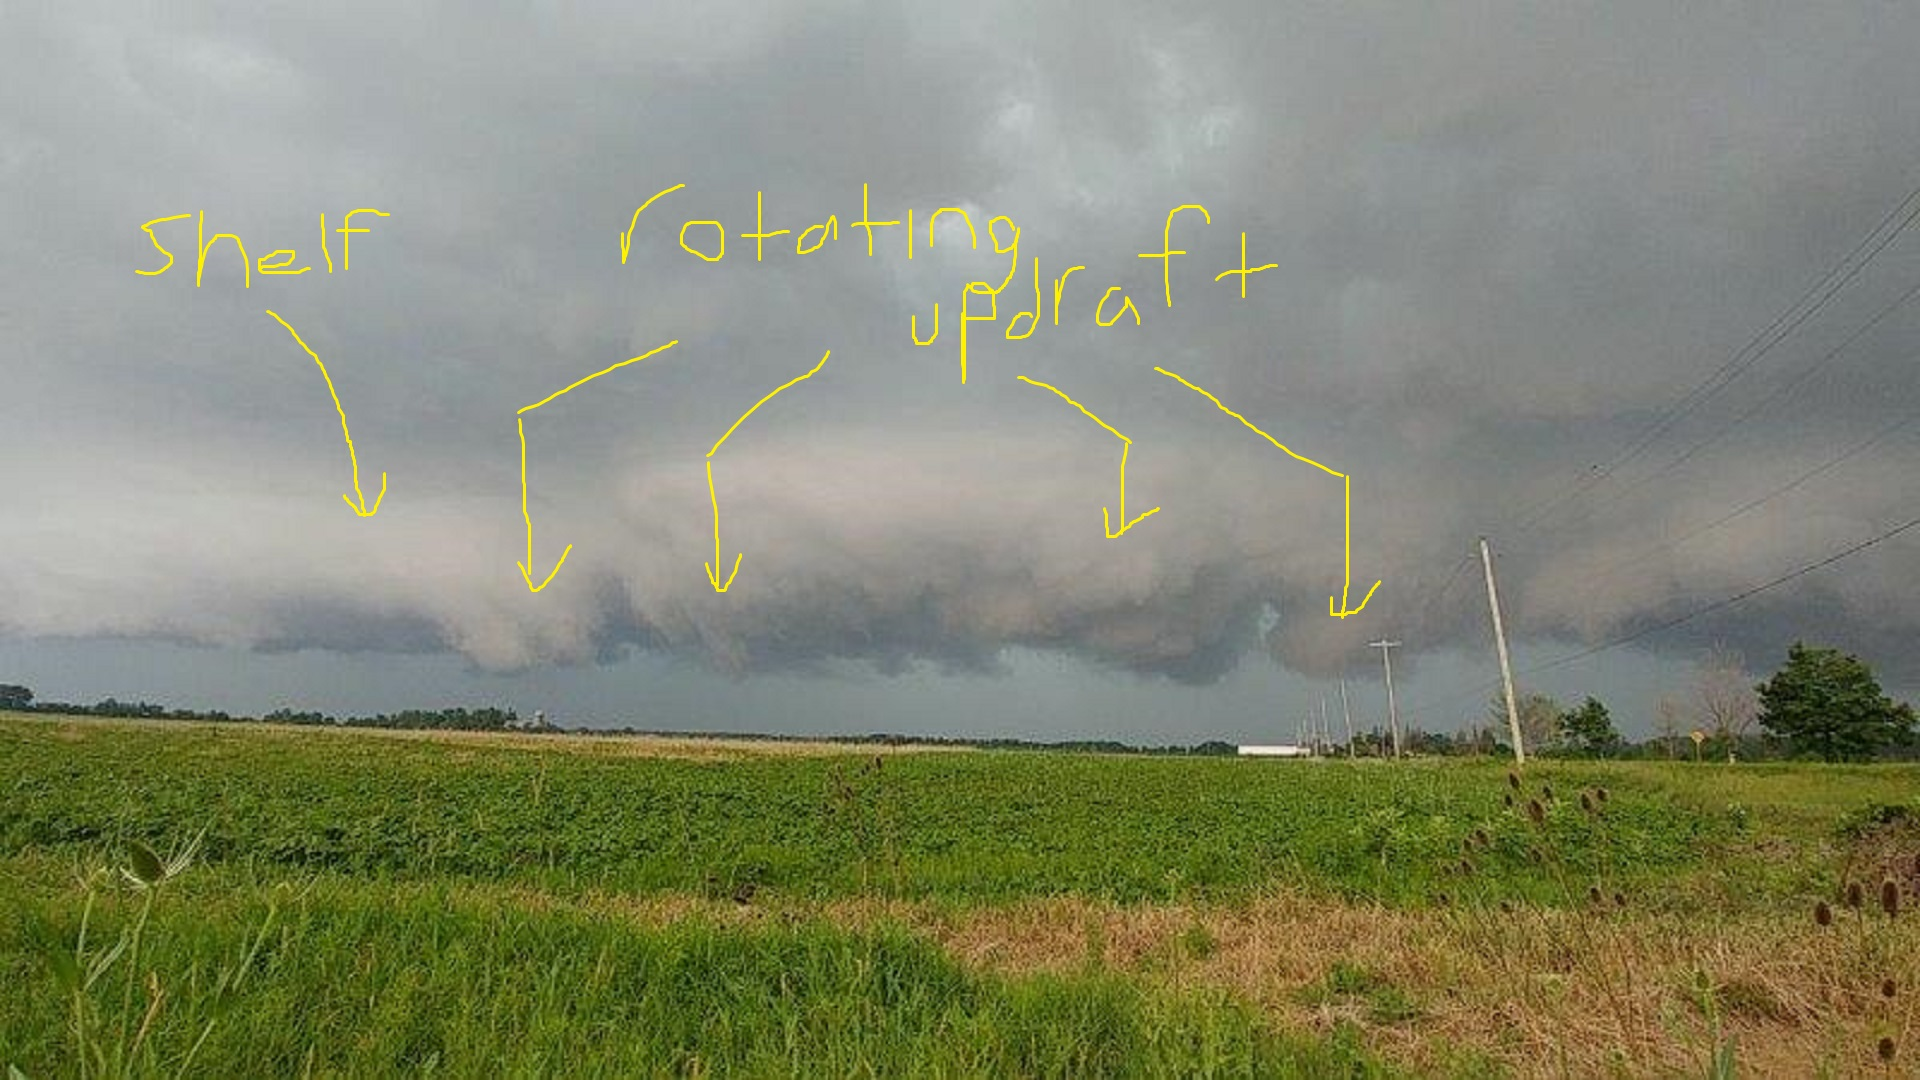
\includegraphics[width=0.8\textwidth]{Weather pics/WS9.jpg}
    \caption{Collision of Two Storms (I)} \label{fig:WS9}
\end{figure}
\noindent

\begin{figure}[H]
    \centering
    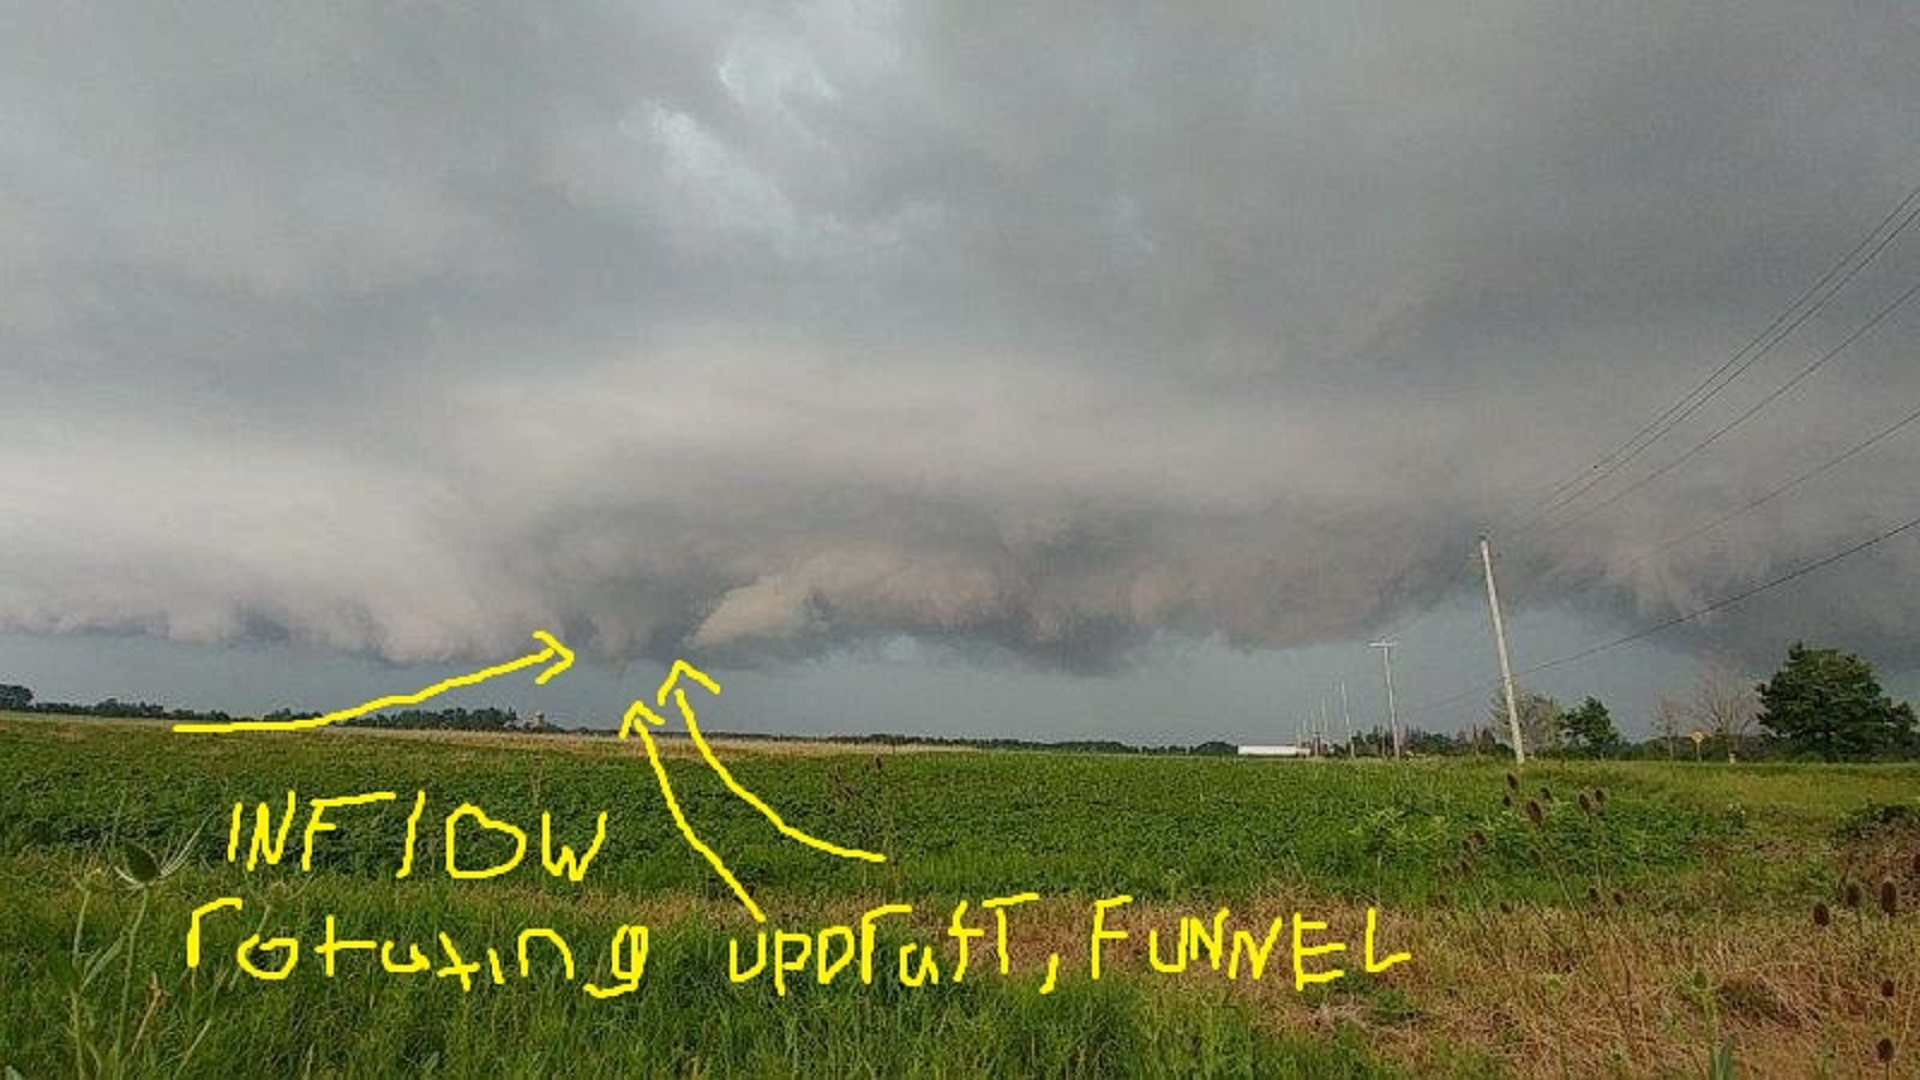
\includegraphics[width=0.8\textwidth]{Weather pics/WS10.jpg}
    \caption{Collision of Two Storms (II)} \label{fig:WS10}
\end{figure}
\noindent

After performing DMD on 73 frames, which has a rank of 73, the
output has dimension 14 given by 14 eigenvalues. We here let the code
determine the optimal dimension. the eigenvalues are in Figure (\ref{fig:WS11}) below. The eigenvalues are plotted on the unit circle.

\begin{figure}[H]
    \centering
    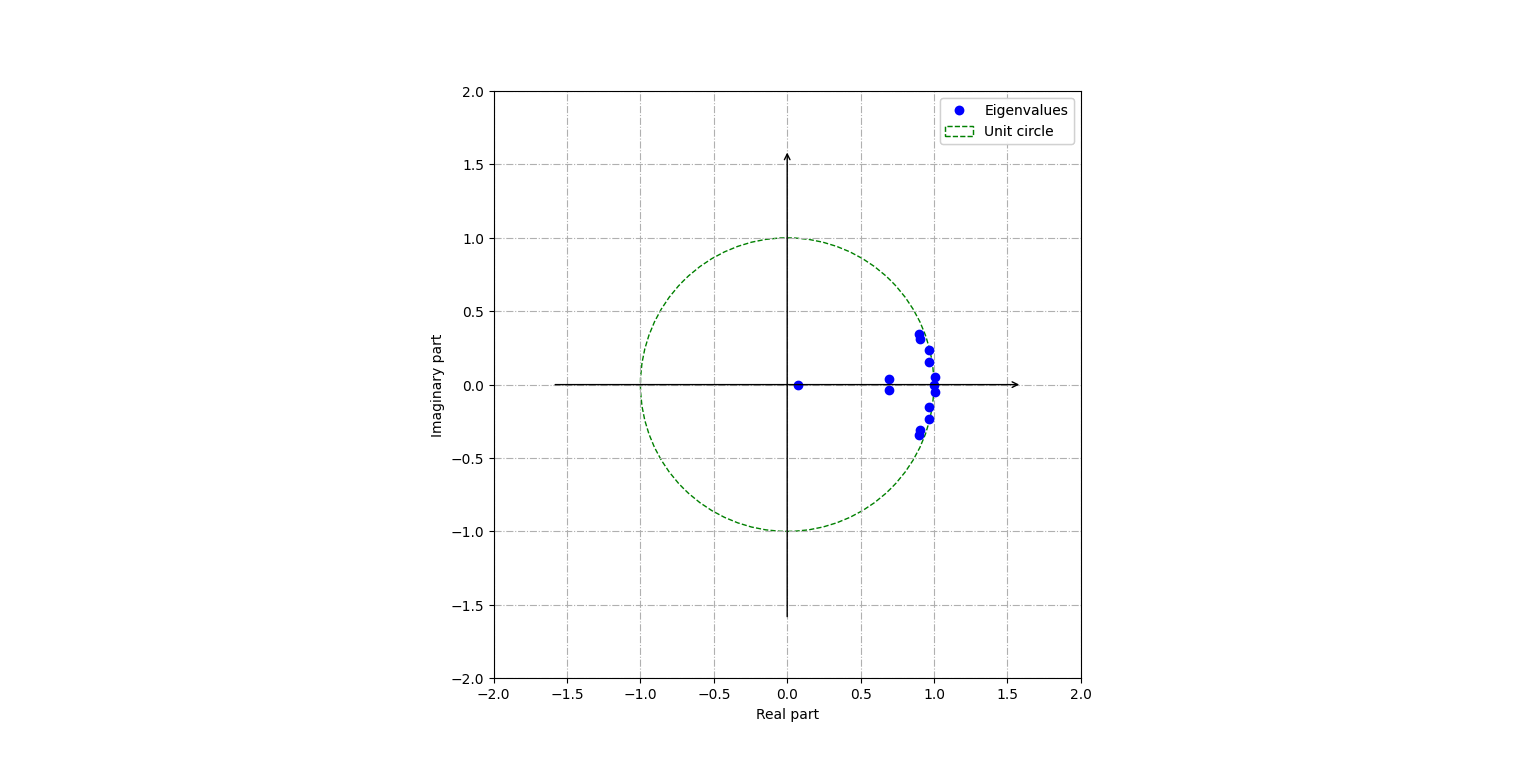
\includegraphics[width=1.3\textwidth]{Weather pics/WS11.png}
    \caption{Eigenvalues of Storm Collision} \label{fig:WS11}
\end{figure}
\noindent

In Figure (\ref{fig:WS12}) and (\ref{fig:WS13}) below we have the output of the DMD of dimension 14. The resulting supercell has been smoothed out, in which has left the shelf cloud retained though has lost much of the structure of the rotating updrafts. As we noted before, one of the challenges of DMD is DMD not picking up these subtle small invariances. We would expect the more eigenvalues given the better DMD will be at retaining the structure of the supercell. Notice most of the eigenvalues are positive representing an unstable system. What would happen if we have negative eigenvalues mostly? If we have eigenvalues outside the unit circle the DMD mode is growing and is better at predicting when this happens.

\begin{figure}[H]
    \centering
    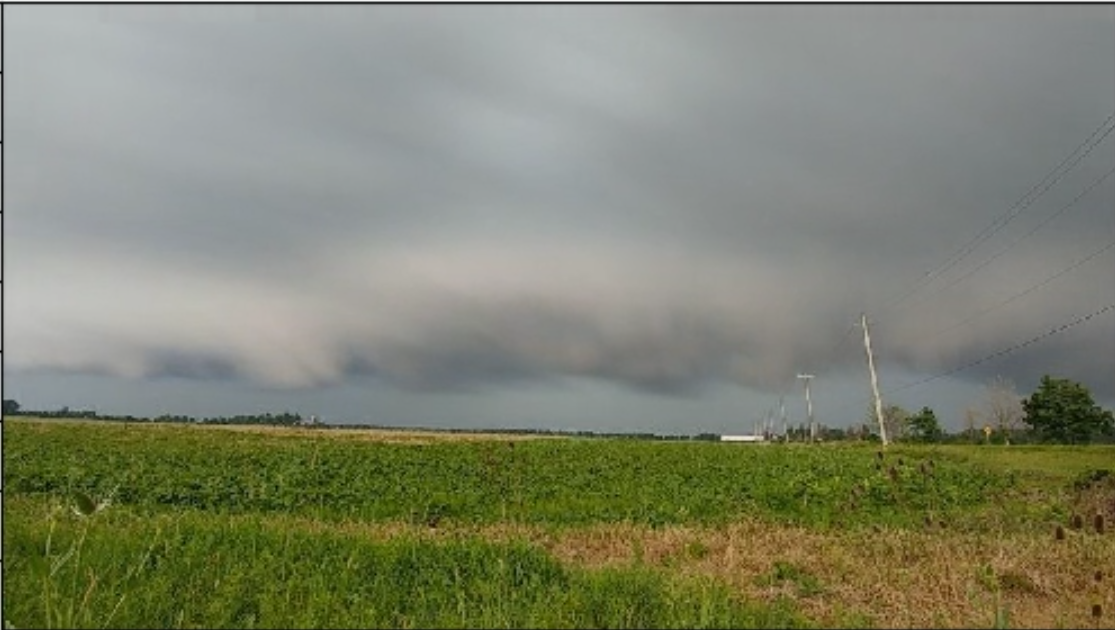
\includegraphics[width=0.8\textwidth]{Weather pics/WS12.png}
    \caption{Frame Produced From DMD With Dimension 14 (I)} \label{fig:WS12}
\end{figure}
\noindent

\begin{figure}[H]
    \centering
    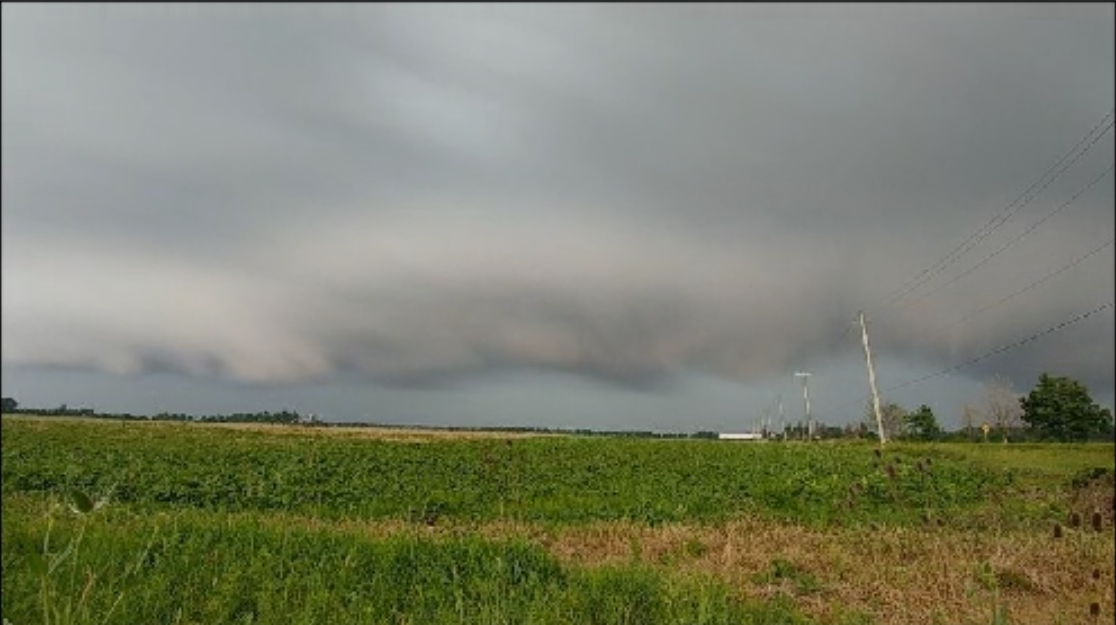
\includegraphics[width=0.8\textwidth]{Weather pics/WS13.png}
    \caption{Frame Produced From DMD With Dimension 14 (II)} \label{fig:WS13}
\end{figure}
\noindent

In Figures (\ref{fig:WS14}) and (\ref{fig:WS15}) below we choose a rank of 60, 60 frames, to see how much structure of the supercell is retained. 

\begin{figure}[H]
    \centering
    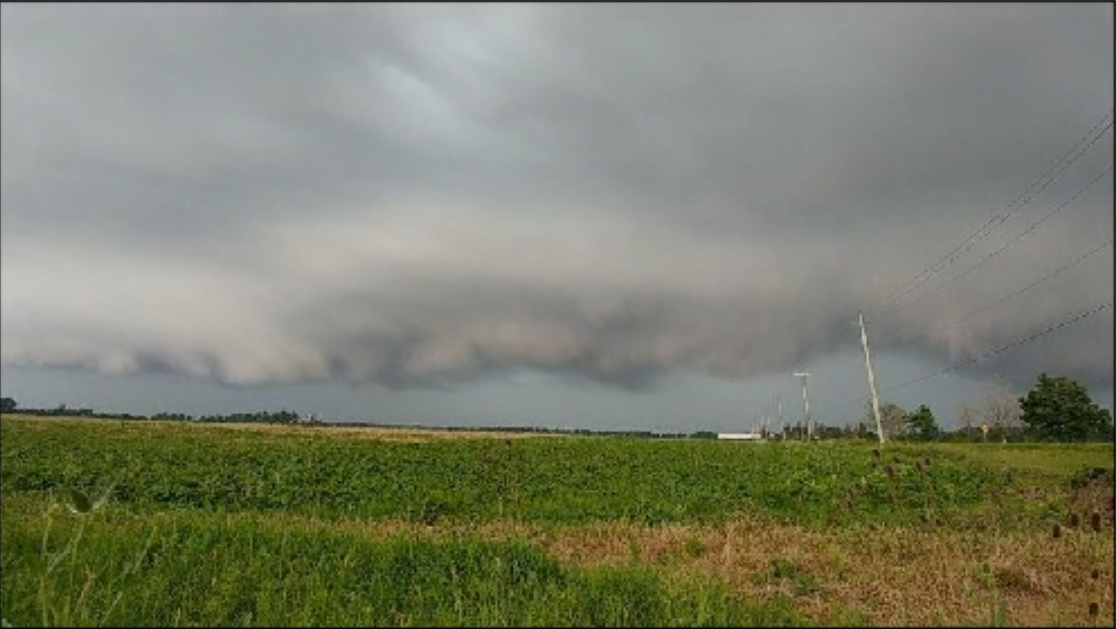
\includegraphics[width=0.8\textwidth]{Weather pics/WS14.png}
    \caption{Frame Produced from DMD With Rank 60 (I)} \label{fig:WS14}
\end{figure}
\noindent

\begin{figure}[H]
    \centering
    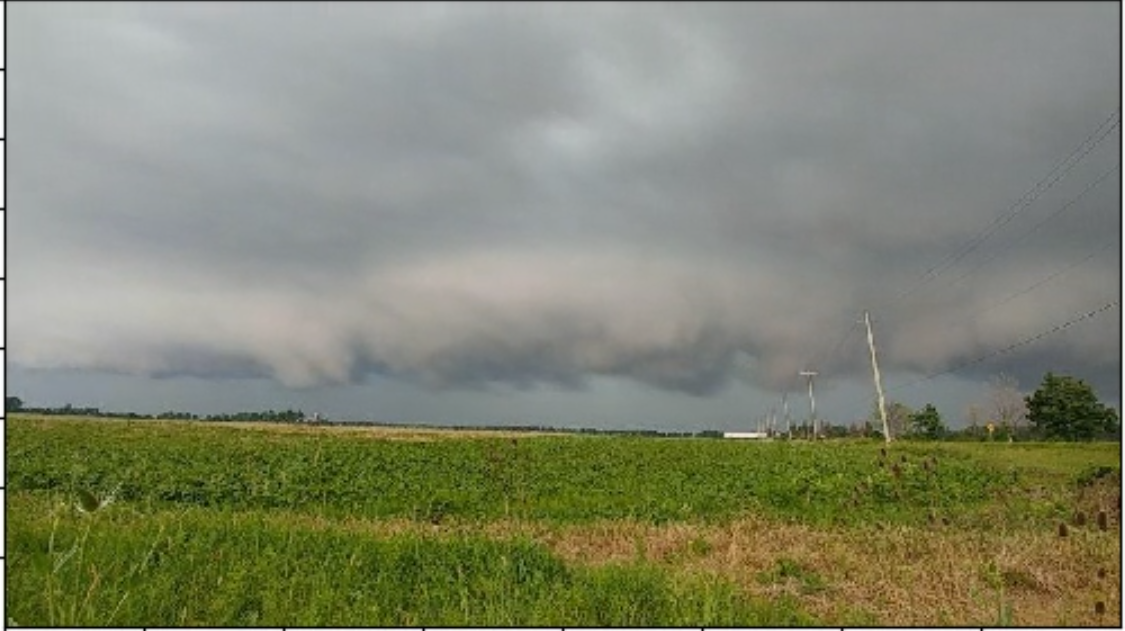
\includegraphics[width=0.8\textwidth]{Weather pics/WS15.png}
    \caption{Frame Produced from DMD With Rank 60 (II)} \label{fig:WS15}
\end{figure}
\noindent

In Figure (\ref{fig:WS16}) below the eigenvalues are depicted which are now more symmetrical, being distributed along the unit circle, as the symmetry of the eigenvalues increases so does the retaining of the structure of the supercell. Here one can clearly see the rotating updrafts vs the one with a rank of 14. One requires great amounts of frames to retain the dynamics of the system, the more data the better. Though we are interested in low-dimensional representations which keep the same structure. More data is computation intensive and we are looking for a lower dimensional algorithm that retains the structure. This is one of the challenges of DMD, lower dimensional representation losing the subtle invariances. If a low dimensional representation of the dynamical system exists then the DMD algorithm would pick it up and retain the same structure as the original. Taking the contra-positive of the statement, Not a representation of the dynamical system implies a low dimensional representation of the system does not exist, hence loss of the structure. Though given the challenges of DMD the above statement applies when the DMD algorithm can identify invariances in the system along with other dynamics. As the rank increases to be close to the number of frames given, the eigenvalues distribute more symmetrically around the circle, hence a neutrally stable system. When we try to predict the future the DMD will produce a periodic extrapolation which is not very useful.

\begin{figure}[H]
    \centering
    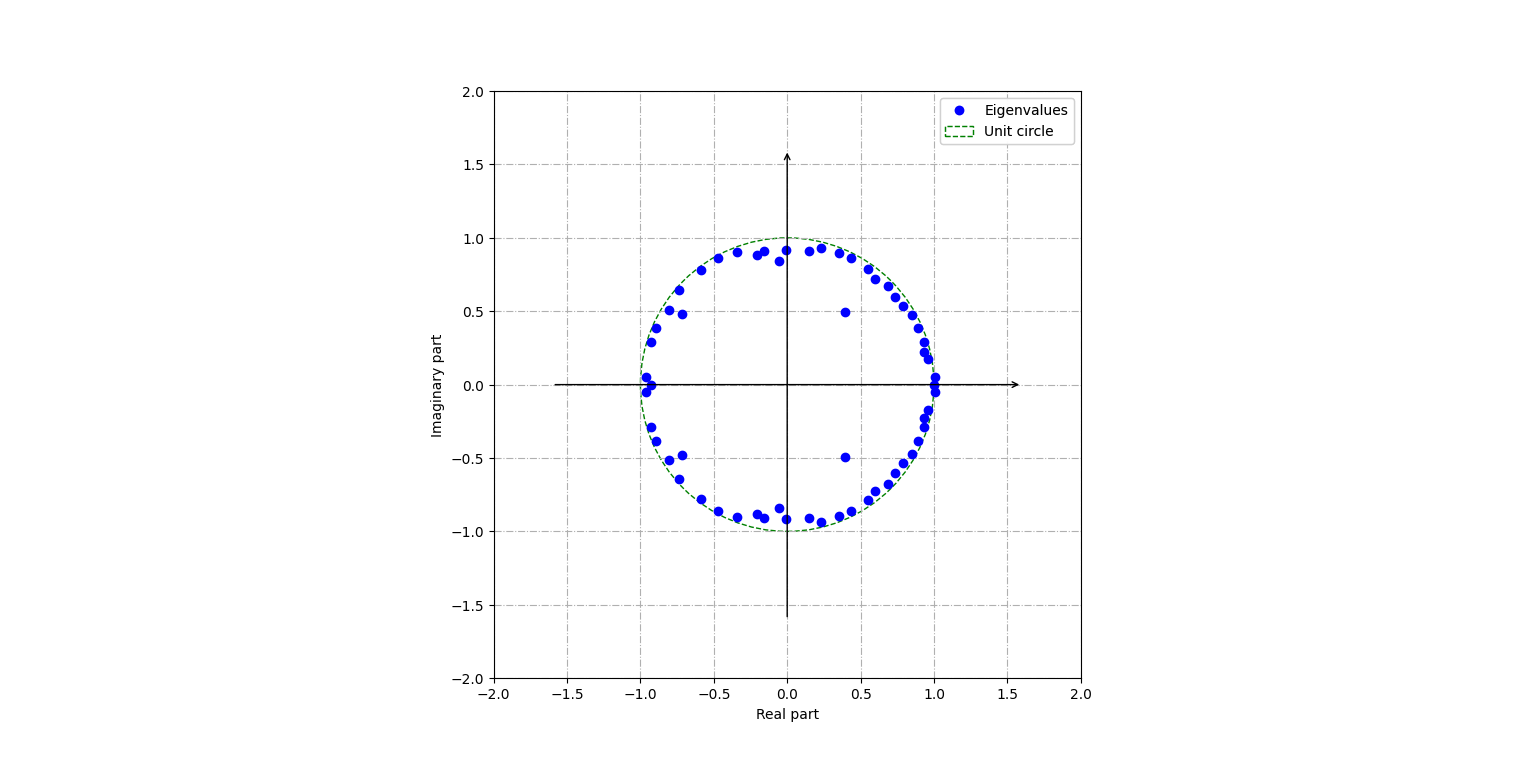
\includegraphics[width=1.3\textwidth]{Weather pics/WS16.png}
    \caption{Updated Eigenvalues of Storm Collision} \label{fig:WS16}
\end{figure}
\noindent

Next, we try to predict the future of the supercell by running DMD on the
movie plus one full length of the movie time into the future. In Figures (\ref{fig:WS17}) through (\ref{fig:WS20}) an image is presented at the final frame, and images after the final frame.

\begin{figure}[H]
    \centering
    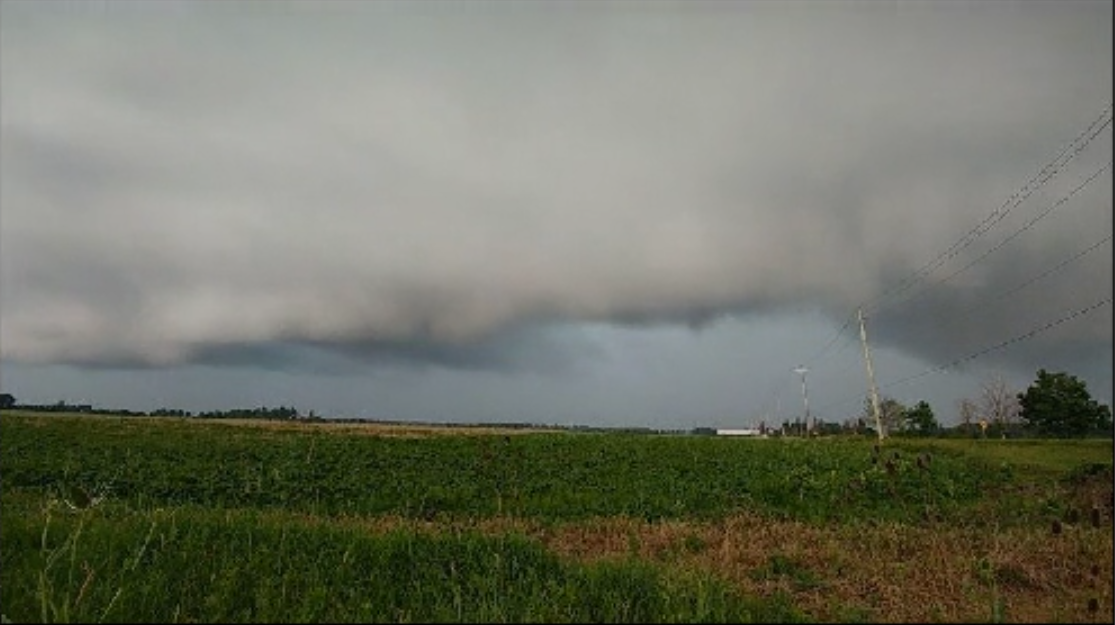
\includegraphics[width=0.8\textwidth]{Weather pics/WS17.png}
    \caption{Future Frame Produced by DMD (I)} \label{fig:WS17}
\end{figure}
\noindent

\begin{figure}[H]
    \centering
    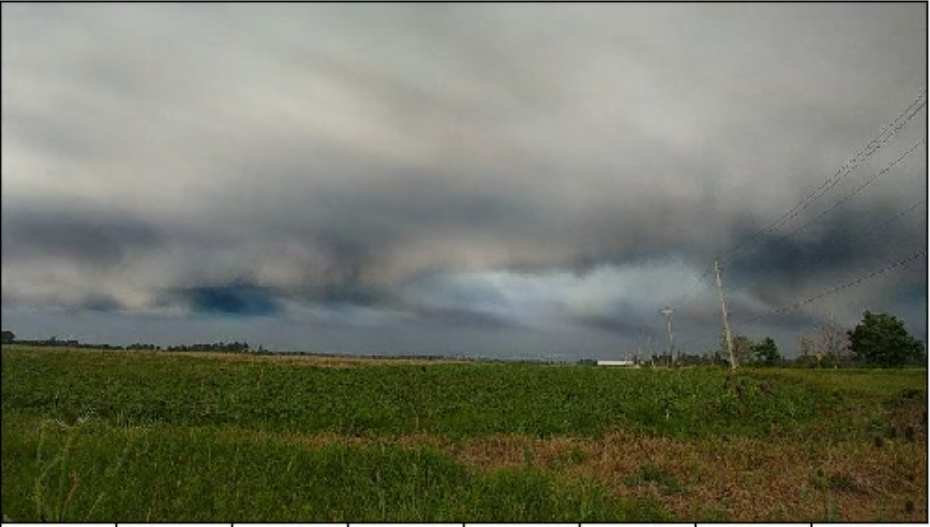
\includegraphics[width=0.8\textwidth]{Weather pics/WS18.png}
    \caption{Future Frame Produced by DMD (II)} \label{fig:WS18}
\end{figure}
\noindent

\begin{figure}[H]
    \centering
    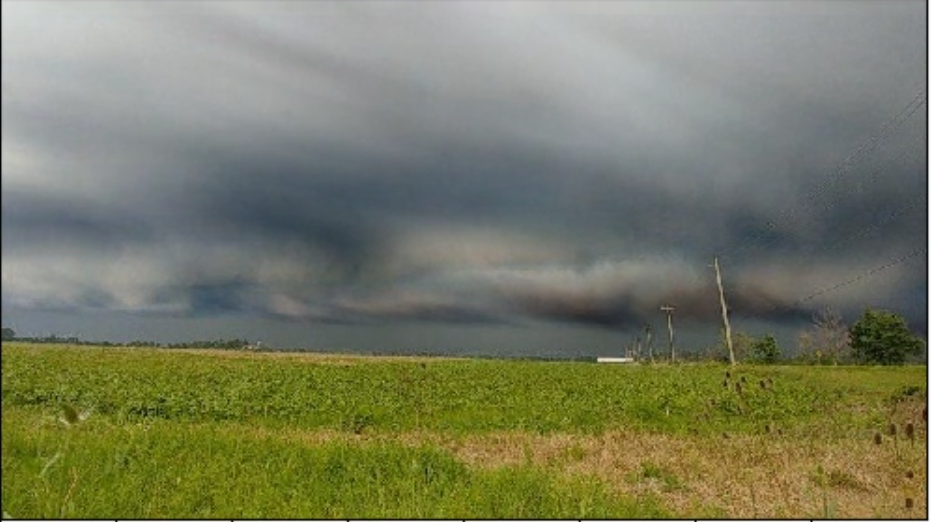
\includegraphics[width=0.8\textwidth]{Weather pics/WS19.png}
    \caption{Future Frame Produced by DMD (III)} \label{fig:WS19}
\end{figure}
\noindent

\begin{figure}[H]
    \centering
    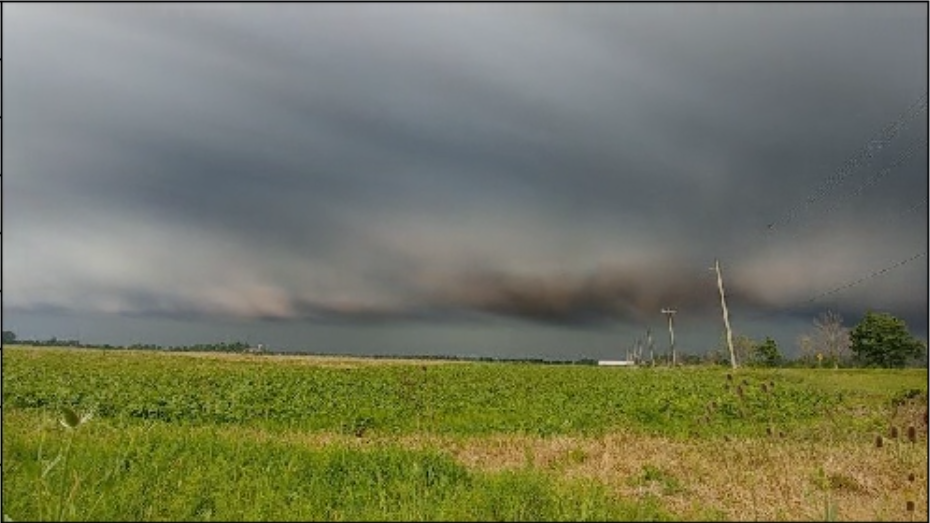
\includegraphics[width=0.8\textwidth]{Weather pics/WS20.png}
    \caption{Future Frame Produced by DMD (IV)} \label{fig:WS20}
\end{figure}
\noindent

We see in Figures (\ref{fig:WS17}) through (\ref{fig:WS20}), The motion of the main supercell has stopped though the DMD is still working within the boundaries given.

\section{Fluid Dynamics}

Then, we apply DMD to water flowing over rocks to simulate turbulence and see how it predicts future scenarios. Given 13 frames of data, we apply DMD specified with a rank of 13. The eigenvalues are depicted below in Figure (\ref{fig:FD1})

\begin{figure}[H]
    \centering
    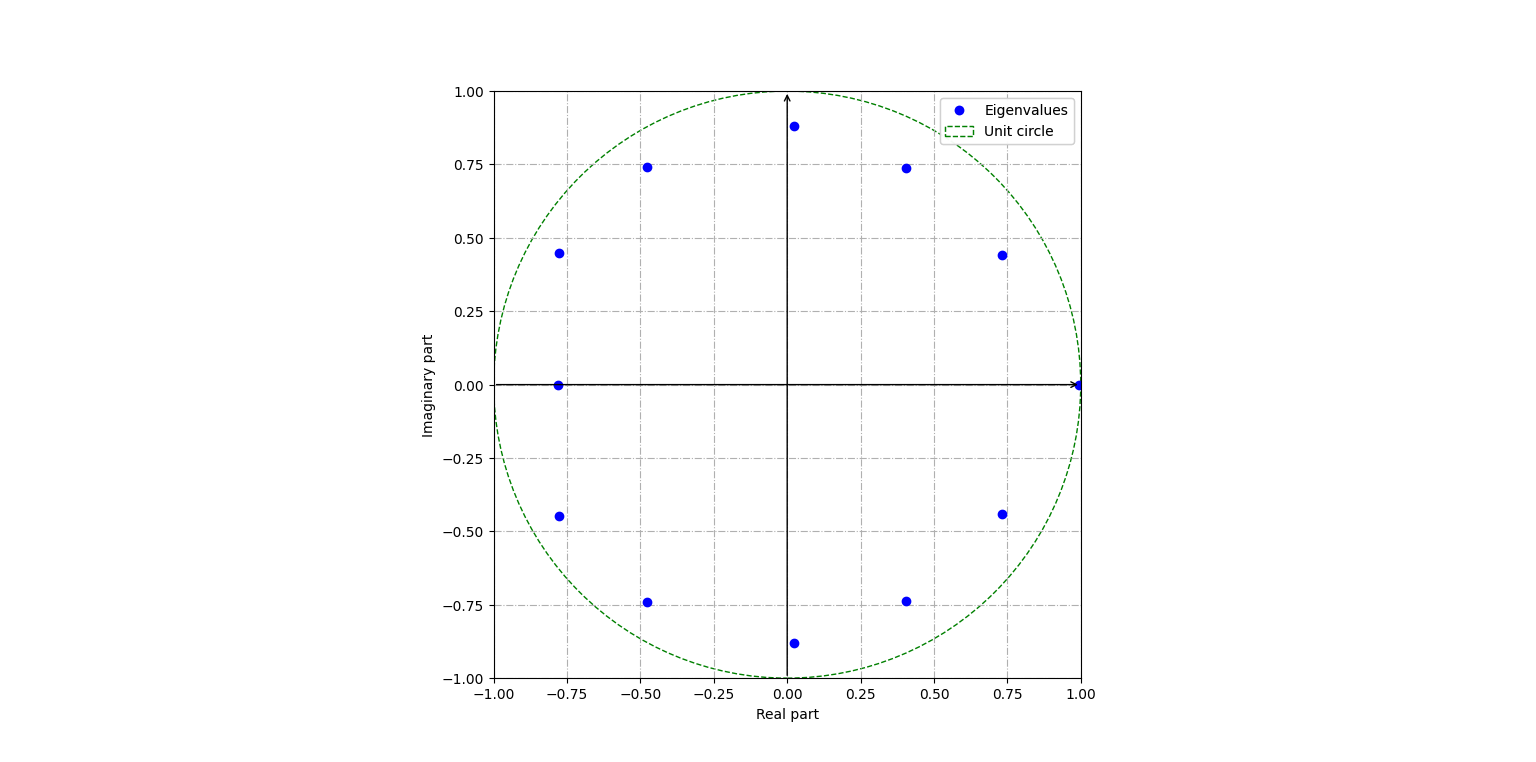
\includegraphics[width=0.8\textwidth]{Fluid Dynamics/FD1.png}
    \caption{Eigenvalues of Water Flow} \label{fig:FD1}
\end{figure}
\noindent
Notice this time we have eigenvalues that are symmetrical due to the full
rank we specified. The DMD mode is decaying and oscillatory. Below is Figures (\ref{fig:FD2}) through (\ref{fig:FD5}) where Figures (\ref{fig:FD1}) and (\ref{fig:FD5}) are actual frames and
in between those is the interpolation between the two frames produced by DMD.

\begin{figure}[H]
    \centering
    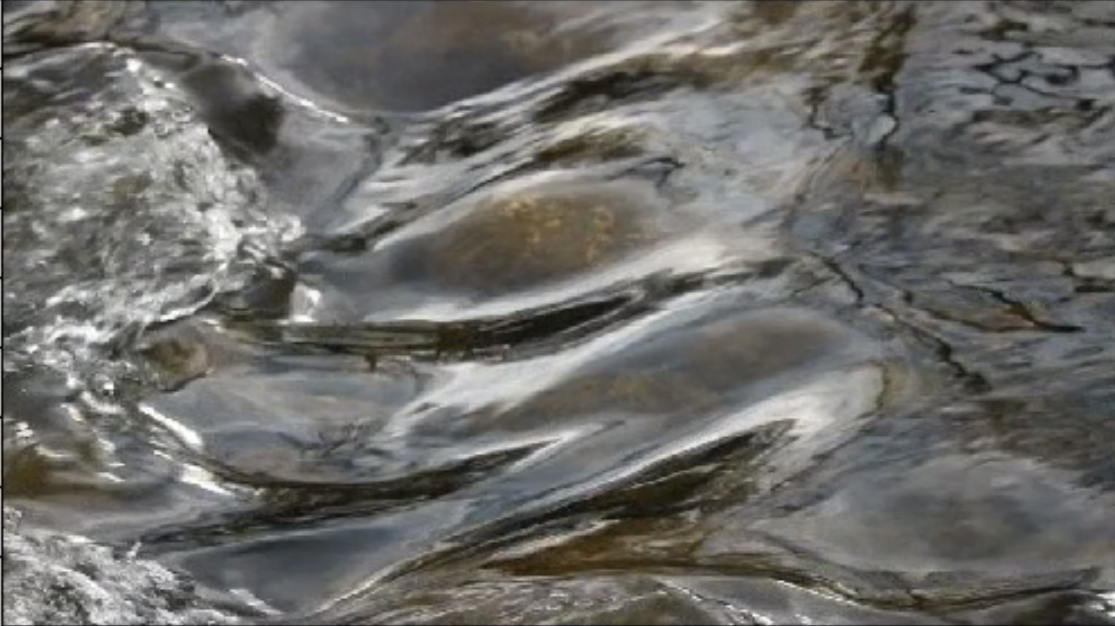
\includegraphics[width=0.8\textwidth]{Fluid Dynamics/FD2.png}
    \caption{Initial Frame of Water Flow From Recording} \label{fig:FD2}
\end{figure}
\noindent

\begin{figure}[H]
    \centering
    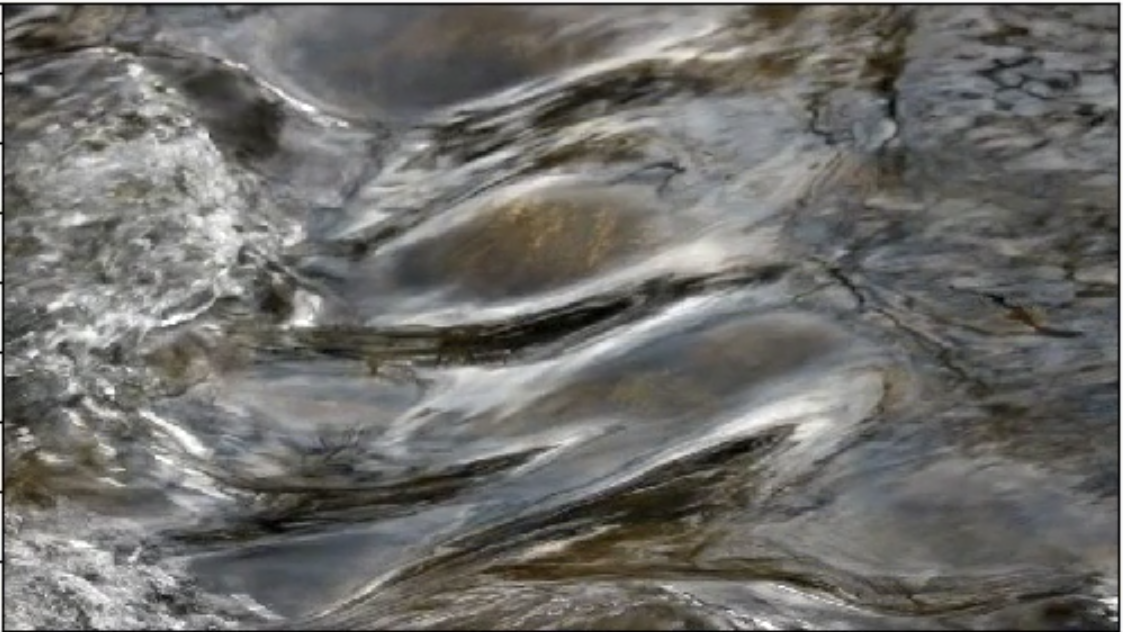
\includegraphics[width=0.8\textwidth]{Fluid Dynamics/FD3.png}
    \caption{Frame Produced by DMD (I)} \label{fig:FD3}
\end{figure}
\noindent

\begin{figure}[H]
    \centering
    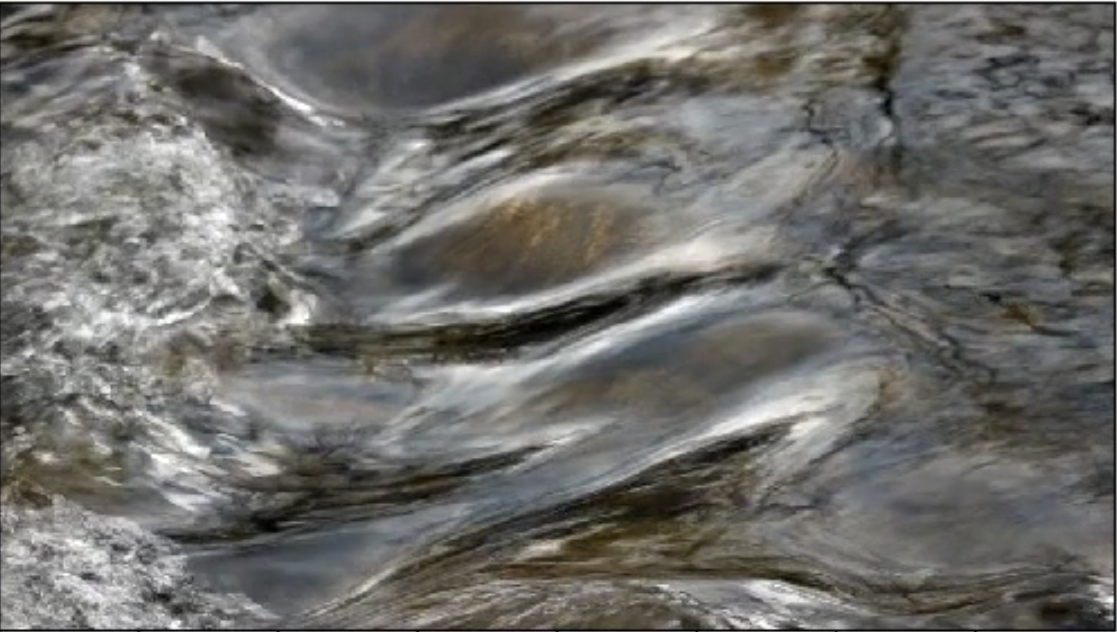
\includegraphics[width=0.8\textwidth]{Fluid Dynamics/FD4.png}
    \caption{Frame Produced by DMD (II)} \label{fig:FD4}
\end{figure}
\noindent

\begin{figure}[H]
    \centering
    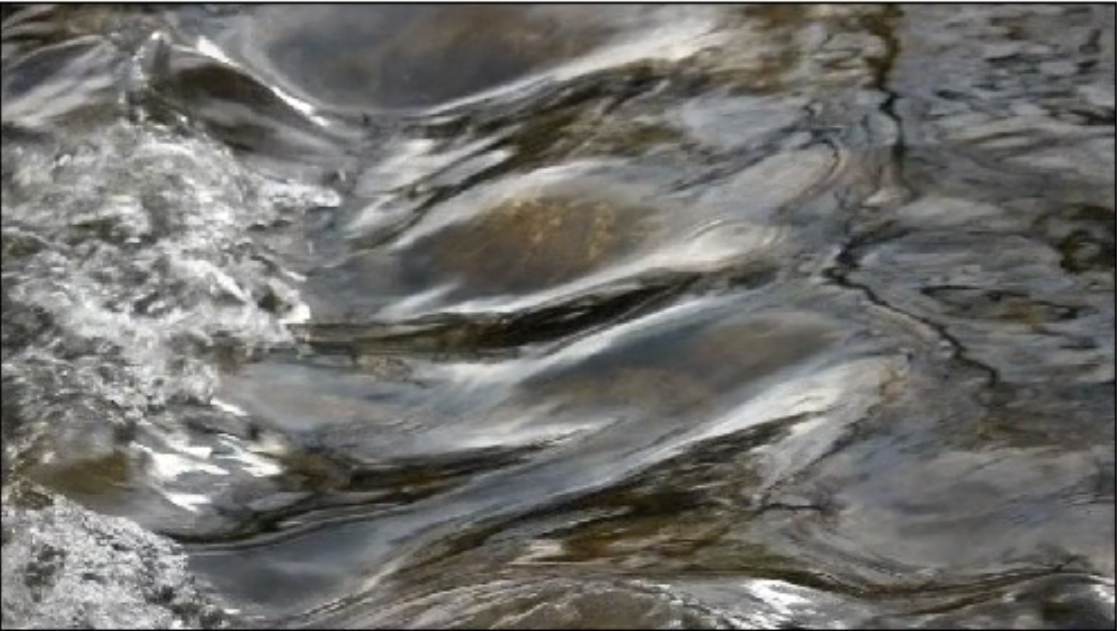
\includegraphics[width=0.8\textwidth]{Fluid Dynamics/FD5.png}
    \caption{Final Frame of Water Flow From Recording} \label{fig:FD5}
\end{figure}
\noindent

Next, we list Figures (\ref{fig:FD6}) through (\ref{fig:FD9}) where these figures occur after the last photo has stopped and it is predicting future outcomes, up to double the length of the time of the original video. We see here now the DMD is predicting outcomes of the turbulence and is not picking up the almost laminar flow before the turbulence. The frames do not pick up the almost laminar flow and images appear to shift around vs flow. We recognized that DMD is not picking up some invariances, being the laminar flow. Given that laminar flow in the system has a consistent pixel intensity between frames it is not surprising that it is not picking up this invariance. Given the symmetrical nature of the eigenvalues, the prediction is periodic and decaying. This is not useful for future predictions.

\begin{figure}[H]
    \centering
    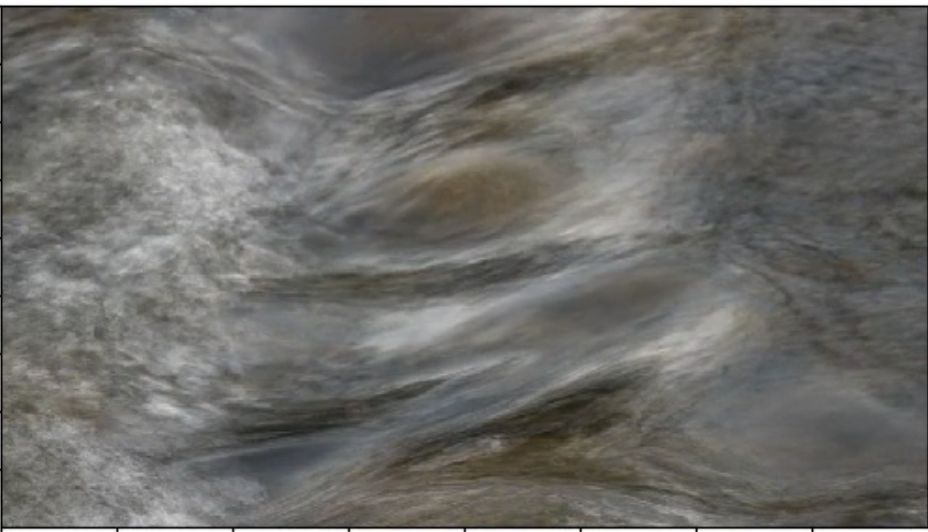
\includegraphics[width=0.8\textwidth]{Fluid Dynamics/FD6.png}
    \caption{Future Frame Produced by DMD (I)} \label{fig:FD6}
\end{figure}
\noindent

\begin{figure}[H]
    \centering
    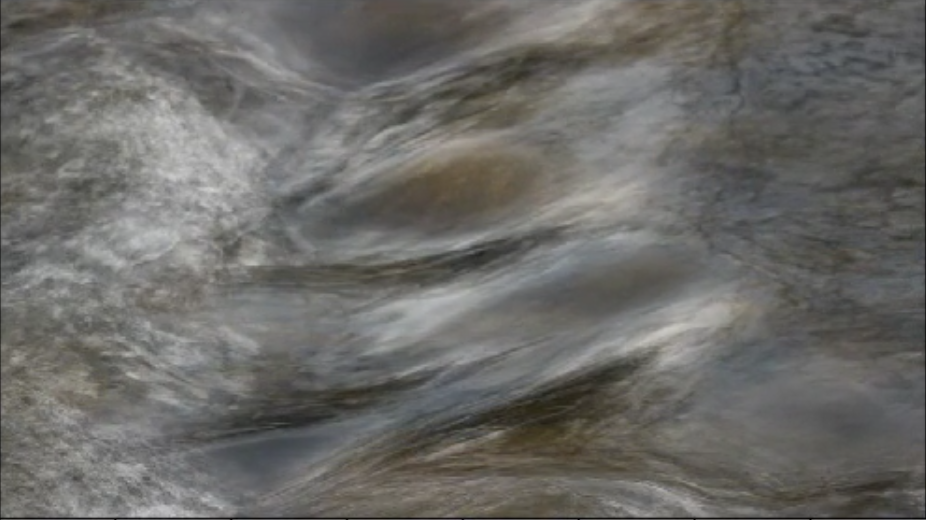
\includegraphics[width=0.8\textwidth]{Fluid Dynamics/FD7.png}
    \caption{Future Frame Produced by DMD (II)} \label{fig:FD7}
\end{figure}
\noindent

\begin{figure}[H]
    \centering
    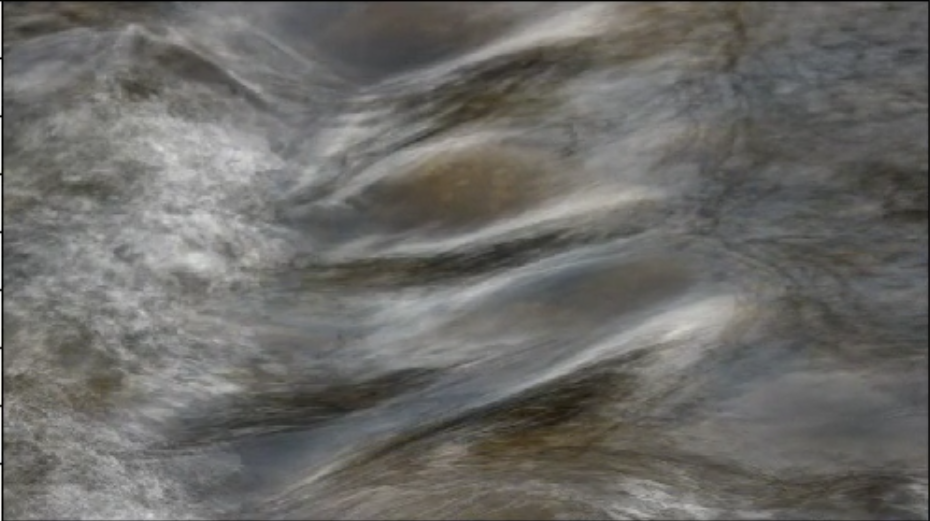
\includegraphics[width=0.8\textwidth]{Fluid Dynamics/FD8.png}
    \caption{Future Frame Produced by DMD (III)} \label{fig:FD8}
\end{figure}
\noindent

\begin{figure}[H]
    \centering
    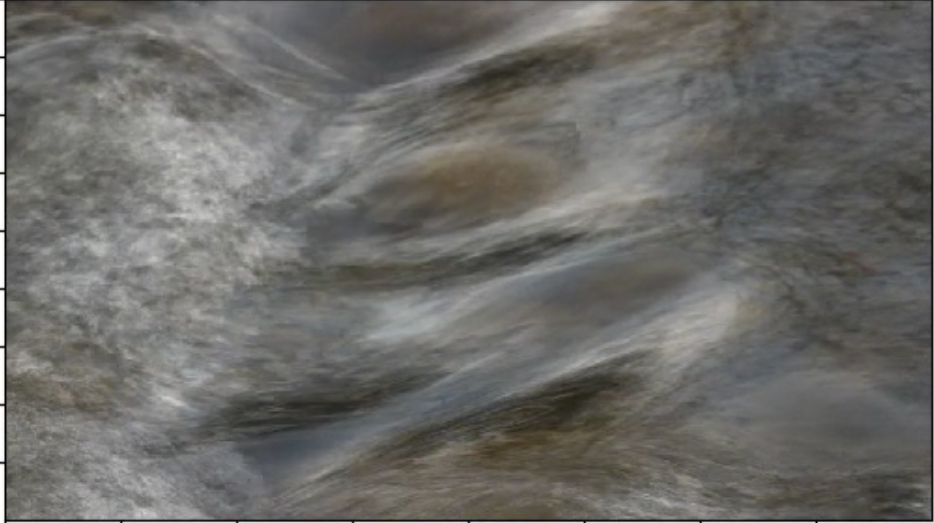
\includegraphics[width=0.8\textwidth]{Fluid Dynamics/FD9.png}
    \caption{Future Frame Produced by DMD (IV)} \label{fig:FD9}
\end{figure}
\noindent

\chapter{Conclusion}

Dynamic mode decomposition (DMD) is a data-analyzation method that applies to a broad range of areas. It organized the data into two large matrices that share the same time interval but with different time stamps, then attempts to generate a mapping from one matrix to the next. Since the matrix can have an enormous amount of elements, DMD utilized the idea of dimensional reduction from singular value decomposition (SVD) for manageable calculations. From the sub-matrices decomposed in SVD, DMD reduces the dimension of the mapping by reformulating and reconstructing the data through its mode. Then from the DMD modes, we can predict the future data at a specific time frame.

This technique can be applied to a host of fields, two of which we studied were how to model infectious disease spread and how to develop financial trading strategies using it. It is clear from the examples above that the algorithm yielded high value information in both cases. In the case of the epidemiology example DMD automatically recognizes the importance of the yearly cycle, providing insight into how the dynamic pattern of the associated mode spreads across a spatial domain. In developing a financial trading strategy DMD was able to produce a strategy that was able to generate profits well above holding stock in the S$\&$P500. 

However, as with everything else DMD has its limitations, one such issue with data-driven, equation-free methods like DMD is that they are limited by the quality and quantity of the data. Another of DMD's limitations is in predicting the future, as seen in the weather systems and fluid dynamics examples. Given the reduced dimension matrices, it can be difficult for computers to calculate as regenerating the data after the reconstruction process, the computer would have to regenerate the same amount of elements back by the end of the process. For the example of frames, although we can reduce the dimension to the number of frames, which is significantly smaller than the number of pixels per frame, we regenerate the same amount of pixels back to each time frame. Additionally, DMD does not capture invariances well. Rotations, translations and other types of low dimensional outputs pick out dominant movement yet miss the subtle invariances. A chaotic system that evolves over time will change and depends on these invariances, hence the system will change from the DMD output over time. 

To improve DMD, we can introduce a controlling matrix to the system that acts on the matrix calculation. In the stance of snapshots, we can use a control to steer the snapshots by way of a set of snapshots and a controlling matrix that acts on the usual snapshots and matrix we have. 

Additionally, introducing analytic solutions of integral systems that approximate the system for a certain time or studying the geometry of fixed rank matrices in order to establish a control to steer the system. It has been conjectured that Maxwell's equations could be investigated to approximate the governing equations of fluid dynamics. Here we are studying the manifold of fixed rank matrices, we could embed this in a higher dimension and project it onto another manifold of known symmetry, analyze the system, and pull it back to the original manifold to try and establish a control to steer system for a certain period of time. Given there is no analytical solution for the Navier-Stokes equations, multiple manifolds will have to be used with a given symmetry to approximate the Navier-Stokes equations, as an evolving system could change the type of symmetry it has as time progresses. 

Another improvement is to have a relation between pixel density and governing equations to be able to incorporate noticing symmetries via DMD in the system. An example is the laminar flow of water, DMD would see that as stationary since the laminar flow does not look like its moving. 

To conclude, although Dynamic Model Decomposition is applicable given a set of data, it is computationally intensive. However, some strategies involve the use of tensor products of matrices to reduce computational time.

\chapter{Algorithm} 
\begin{lstlisting}[language=python]
!pip install scipy
!pip install matplotlib
import os

import matplotlib.pyplot as plt
import warnings
import scipy
warnings.filterwarnings('ignore')

!pip install pydmd
!pip install pykoopman

from pydmd import DMD
from matplotlib import animation
from IPython.display import HTML
from imageio import imread
import numpy as np
from os import listdir
import pykoopman as pk
from pydmd import DMDc
from pydmd import DMD, SubspaceDMD
from pydmd import HODMD
from google.colab import files
uploaded = files.upload()
os.chdir('/content/june29/')

frames = os.listdir('/content/june29/')
vectorized_frames = []

for frame in frames:
    vectorized_picture = 
    np.array(imread("/content/june29/" + frame).flatten())
    # reshaped_vectorized_picture = 
    vectorized_picture.reshape(1, -1).T
    vectorized_frames.append(vectorized_picture)

vectorized_frames = np.array(vectorized_frames)

print(vectorized_frames)

dmd = DMD(svd_rank=35)
dmd.fit(vectorized_frames.T/255)
dmdc = DMD(svd_rank=35,tlsq_rank=20)
#dmd3 = HODMD(svd_rank=12,d=1)
#dmd3.fit(vectorized_frames.T/255)
#dmd3.plot_eigs()
#dmdc = DMDc(svd_rank=35,tlsq_rank=10)
#dmdc.fit(vectorized_frames.T/255, np.random.rand(34, 34))
dmdc.fit(vectorized_frames.T/255)
for eig in dmd.eigs:
     print('Eigenvalue {}: distance from unit circle {}'.format(eig,
     np.abs(np.sqrt(eig.imag**2+eig.real**2) - 1)))
for eig in dmdc.eigs:
     print('Eigenvalue {}: distance from unit circle {}'.format(eig,
     np.abs(np.sqrt(eig.imag**2+eig.real**2) - 1))) 
#for eig in dmd3.eigs:
    #print('Eigenvalue {}: distance from unit circle {}'.format(eig,
    np.abs(np.sqrt(eig.imag**2+eig.real**2) - 1)))        

dmd.plot_eigs(show_axes=True, show_unit_circle=True)
dmdc.plot_eigs(show_axes=True, show_unit_circle=True)
#dmd3.plot_eigs(show_axes=True, show_unit_circle=True)

dmd.dmd_time['dt'] *= .10
dmd.dmd_time['tend'] *=2
dmdc.dmd_time['dt'] *= .10
dmdc.dmd_time['tend'] *=2
# dmd3.dmd_time['dt'] *= .10
# dmd3.dmd_time['tend'] *=1

fig = plt.figure()

out = [[plt.imshow(state.reshape(450, 800, 3), 
interpolation='nearest')] 
for state in np.abs(dmd.reconstructed_data.T)]

ani = animation.ArtistAnimation(fig,out,
interval=500*dmd.dmd_time['dt'],blit=False)

ani.save('interp.mp4')


plt.show()

out1 = [[plt.imshow(state.reshape(450, 800, 3),
interpolation='nearest')] 
for state in np.abs(dmdc.reconstructed_data.T)]
ani1 = animation.ArtistAnimation(fig,out,
interval=500*dmdc.dmd_time['dt'],blit=False)
ani1.save('interp1.mp4')
plt.show()

# out2 = [[plt.imshow(state.reshape(450, 800, 3), interpolation=
'nearest')] for state in 
np.abs(dmd3.reconstructed_data)]
# ani2 = animation.ArtistAnimation(fig,out2,
interval=3000*dmd3.dmd_time['dt'],blit=False)
# ani2.save('interp2.mp4')
# plt.show()

#DMD.plot_snapshots_2D(, index_snap=None)
#####################################################
\end{lstlisting}

\begin{thebibliography}{9}
\bibitem{DMDMSc}
Muniraju A, (2018) 
\textit{Analysis of Dynamic Mode Decomposition},
Theses and Dissertations, 1879.

\bibitem{DMDbook}
Kutz JN, Brunton SL, Brunton BW, et al. (2016) 
\textit{Dynamic Mode Decomposition: Data-Driven Modeling of Complex Systems}, Philadelphia, PA, Society for Industrial and Applied Mathematics.

\bibitem{Epidemiology}
Proctor JL, Eckhoff PA, (2015) \textit{Discovering dynamic patterns from infectious disease data using dynamic mode decomposition.} International Health 7: 139–145.

\bibitem{GFT} 
Google flu trends estimates \url{https://www.google.com/publicdata/explore?ds=z3bsqef7ki44ac_#!ctype=l&amp;strail=false&amp;bcs=d&amp;nselm=h&amp;met_y=flu_index&amp;scale_y=lin&amp;ind_y=false&amp;rdim=region&amp;idim=region:US-AL:US-AK:US-AZ:US-AR:US-CA:US-CO:US-CT:US-DE:US-DC:US-FL:US-GA:US-HI:US-ID:US-IL:US-IN:US-IA:US-KS:US-KY:US-LA:US-ME:US-MD:US-MA:US-MI:US-MN:US-MS:US-MO:US-MT:US-NE:US-NV:US-NH:US-NJ:US-NM:US-NY:US-NC:US-ND:US-OH:US-OK:US-WY:US-WI:US-WV:US-WA:US-VA:US-VT:US-UT:US-TX:US-TN:US-OR:US-PA:US-RI:US-SC:US-SD&amp;ifdim=region:country:US&amp;tstart=1183003200000&amp;tend=1438833600000&amp;hl=en_US&amp;dl=en_US&amp;ind=false} (accessed Nov 1, 2022). 

\bibitem{Financial}
Mann J, Kutz JN, (2016) 
\textit{Dynamic mode decomposition for financial trading strategies.} Quantitative Finance 16: 1643–1655.

\end{thebibliography}


\end{document}
